% Created 2023-04-02 Κυρ 12:03
% Intended LaTeX compiler: pdflatex
\documentclass[11pt]{article}
\usepackage[utf8]{inputenc}
\usepackage[T1]{fontenc}
\usepackage{graphicx}
\usepackage{longtable}
\usepackage{wrapfig}
\usepackage{rotating}
\usepackage[normalem]{ulem}
\usepackage{amsmath}
\usepackage{amssymb}
\usepackage{capt-of}
\usepackage{hyperref}
\usepackage{booktabs}
\usepackage{import}
\usepackage[LGR, T1]{fontenc}
\usepackage[greek, english]{babel}
\usepackage{alphabeta}
\usepackage{esint}
\usepackage{mathtools}
\usepackage{esdiff}
\usepackage{makeidx}
\usepackage{glossaries}
\usepackage{newfloat}
\usepackage{minted}
\usepackage[a4paper, margin=3cm]{geometry}
\usepackage{chemfig}
\usepackage{svg}
\author{Βιδιάνος Γιαννίτσης, Αριστοτέλης Αργυρόπουλος, Θεωφανώ Αντωνία Πόταρη, Στυλιανή Σταύρου}
\date{\today}
\title{Ενεργειακή ολοκλήρωση και Κοστολόγηση}
\hypersetup{
 pdfauthor={Βιδιάνος Γιαννίτσης, Αριστοτέλης Αργυρόπουλος, Θεωφανώ Αντωνία Πόταρη, Στυλιανή Σταύρου},
 pdftitle={Ενεργειακή ολοκλήρωση και Κοστολόγηση},
 pdfkeywords={},
 pdfsubject={},
 pdfcreator={Emacs 28.2 (Org mode 9.5.5)}, 
 pdflang={English}}
\makeatletter
\newcommand{\citeprocitem}[2]{\hyper@linkstart{cite}{citeproc_bib_item_#1}#2\hyper@linkend}
\makeatother

\usepackage[notquote]{hanging}
\begin{document}

\maketitle
\tableofcontents

\renewcommand{\abstractname}{Περίληψη}
\renewcommand{\tablename}{Πίνακας}
\renewcommand{\figurename}{Σχήμα}
\renewcommand\listingscaption{Κώδικας}

\section{Εισαγωγή}
\label{sec:org43ec364}
Στην πρόοδο αυτή εξετάστηκε η ενεργειακή ολοκλήρωση των ρευμάτων και διεργασιών που υπάρχουν, με σκοπό την ελαχιστοποίηση θερμών και ψυχρών παροχών που απαιτούνται. Επίσης, εξετάστηκε και μία πρώτη εικόνα της κοστολόγησης, η οποία βέβαια θα ολοκληρωθεί για την τελική πρόοδο.

\section{Αναγνώριση θερμών και ψυχρών ρευμάτων}
\label{sec:orgea6316c}
Για να γίνει η ενεργειακή ολοκλήρωση, πρέπει πρώτα να αναγνωριστούν όλα τα θερμά και ψυχρά ρεύματα της διεργασίας. Αυτή η διαδικασία γίνεται παρακάτω.

\subsection{Block 100 - Διαχωρισμός των τριών κομματιών της βιομάζας}
\label{sec:orgfbb855f}
Το block αυτό είναι για την βασική διεργασία διαχωρισμού την έκρηξη ατμού και της επακόλουθες διεργασίες διαχωρισμού κυτταρίνης-λιγνίνης. Ως τροφοδοσία έχει νερό για παραγωγή ατμού, πυρηνόξυλο (πρώτη ύλη) και τα υδατικά διαλύματα που απαιτούνται για τις διεργασίες διαχωρισμού. Προιόντα είναι τα τρία βασικά ρεύματα ξυλόζης, κυτταρίνης και λιγνίνης.

\begin{figure}[htbp]
\centering
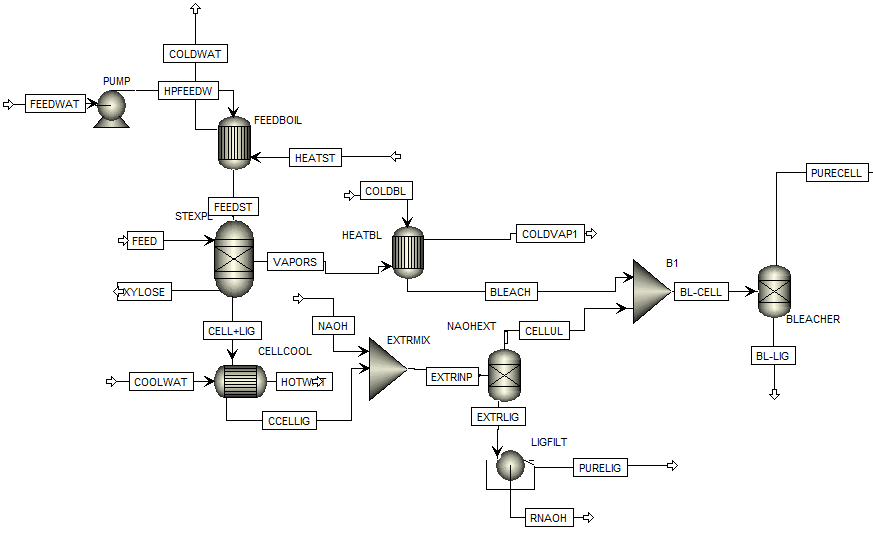
\includegraphics[width=.9\linewidth]{Block_100_-_Διαχωρισμός_των_τριών_κομματιών_της_βιομάζας/2023-03-11_15-21-38_screenshot.png}
\caption{Block 100 στο Aspen}
\end{figure}

Στο block αυτό, έχουμε τα εξής.
\begin{itemize}
\item Aτμός της τροφοδοσίας ο οποίος θερμαίνεται από θερμοκρασία περιβάλλοντος μέχρι 232 \(^oC\) (ψυχρό ρεύμα). Το ρεύμα με το οποίο εναλλάσσει θερμότητα είναι βοηθητική παροχή της διεργασίας. Κάποια από την θερμότητα του προσφέρεται για την θέρμανση και διάσπαση του πυρηνόξυλου, ενώ ο υπόλοιπος ατμός, μαζί με τα υπόλοιπα ατμώδη υπολείμματα της έκρηξης (κυρίως CO\textsubscript{2}) διατίθενται ως ένα θερμό ρεύμα της διεργασίας. Βέβαια, αν παρατηρηθεί πως υπάρχει περίσσεια θερμικής ενέργειας, μπορεί αυτό το ρεύμα να μην χρησιμοποιηθεί.
\item Κυτταρίνη και Λιγνίνη που βγαίνουν από το steam explosion στους 232 και πρέπει να ψυχθούν μέχρι την θερμοκρασία λειτουργίας της αλκαλικής εκχύλισης (80 \(^oC\)). Μπορούμε να εκμεταλλευτούμε το υπάρχον θερμικό περιεχόμενο τους για να θερμάνουμε και το διάλυμα καυστικού νατρίου όμως. Η θερμοκρασία βγαίνει 80.65 \(^oC\) αν ο εναλλάκτης το ψύξει μέχρι τους 105 \(^oC\).
\item Η ξυλόζη οδηγείται στην διεργασία παραγωγής κυκλοπεντανόνης, για αυτό για το block αυτό δεν μεταβάλλεται η θερμότητα της.
\item Θέρμανση του διαλύματος χλωρίνης (bleach) καθώς για την πλήρη απολιγνοποίση θέλουμε εφαρμογή του διαλύματος αυτού στους 70 \(^oC\) (ψυχρό ρεύμα). Στο παρόν διάγραμμα ροής γίνεται εν μέρει με την θερμότητα των ατμών της έκρηξης ατμού και μετά με την ανάμιξη με το ρεύμα κυτταρίνης για τελική θερμοκρασία 69.9 \(^oC\). Στην ανάμιξη αυτή έχουμε και μείωση της θερμότητας του ρεύματος κυτταρίνης κατά 10 \(^oC\) περίπου.

Άρα μπορούμε να κάνουμε τον εξής πίνακα για τα εκμεταλλεύσιμα θερμά και ψυχρά ρεύματα
\end{itemize}

\begin{table}[htbp]
\caption{Θερμά και Ψυχρά Ρεύματα στο Block 100}
\centering
\begin{tabular}{llrrrl}
Ρεύμα & Είδος & Τ\textsubscript{in} (C) & Τ\textsubscript{out} (C) & Παροχή (kmol/hr) & Σύσταση\\
\hline
FeedSteam & Ψυχρό & 20 & 232 & 633.22 & Νερό\\
\hline
Vapors & Θερμό & 232 & 30 & 905.27 & Νερό 0.92\\
 &  &  &  &  & CO\textsubscript{2} 0.08\\
\hline
CellLig & Θερμό & 232 & 80.65 & 84.76 & Κυτταρίνη 0.5\\
 &  &  &  &  & Λιγνίνη 0.5\\
\hline
NaOH & Ψυχρό & 20 & 80.65 & 80.37 & Νερό\\
\hline
Bleach & Ψυχρό & 20 & 69.9 & 55.62 & Νερό 99.5\\
 &  &  &  &  & Χλωρίνη 0.05\\
\hline
Cellulose & Θέρμο & 80.65 & 69.9 & 54.32 & Κυτταρίνη 0.78\\
 &  &  &  &  & Λιγνίνη 0.22\\
\hline
\end{tabular}
\end{table}

\subsection{Block 200 - Παραγωγή Γλυκόζης}
\label{sec:orgece4a5a}
Στο block αυτό θεωρείται ως τροφοδοσία η καθαρή κυτταρίνη του block 100 και νερό το οποίο απαιτείται για την υδρόλυση της κυτταρίνης. Προιόν της διεργασίας είναι η γλυκόζη που θα τροφοδοτηθεί στον βιοαντιδραστήρα παραγωγής γλυκερόλης (block 400).

\begin{figure}[htbp]
\centering
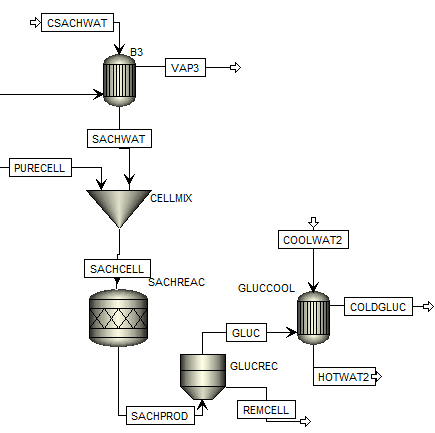
\includegraphics[width=300px]{Block_200_-_Παραγωγή_Γλυκόζης/2023-03-11_16-51-41_screenshot.png}
\caption{Block 200 στο Aspen}
\end{figure}


Στο block αυτό:
\begin{itemize}
\item Θέλουμε η κυτταρίνη και το νερό να τροφοδοτηθούν στους 50 \(^oC\) για την υδρόλυση. Για αυτό, το νερό πρώτα θερμαίνεται μέχρι μία θερμόκρασία και μετά αναμιγνύεται με την κυτταρίνη για τελική θερμοκρασία 49.75 \(^oC\). Το νερό ξεκινάει από θερμοκρασία περιβάλλοντος και θερμαίνεται (επειδή η θερμοκρασία θα πέσει πολύ αν αναμιχθούν ως έχει) ενώ η κυτταρίνη ψύχεται από τους 69.9 \(^oC\).
\item Η γλυκόζη ψύχεται από τους 50 \(^oC\) στους οποίους παράχθηκε μέχρι τους 30 \(^oC\) η οποία είναι η βέλτιστη λειτουργία του αντιδραστήρα παραγωγής γλυκερόλης στο block 400.

Άρα μπορούμε να κάνουμε τον εξής πίνακα για τα εκμεταλλεύσιμα θερμά και ψυχρά ρεύματα
\end{itemize}
\begin{table}[htbp]
\caption{Θερμά και Ψυχρά Ρεύματα στο Block 200}
\centering
\begin{tabular}{llrrrl}
Ρεύμα & Είδος & Τ\textsubscript{in} (C) & Τ\textsubscript{out} (C) & Παροχή (kmol/hr) & Σύσταση\\
\hline
PureCell & Θερμό & 61.97 & 49.75 & 42.55 & Κυτταρίνη\\
\hline
SachWater & Ψυχρό & 20 & 49.75 & 715 & Νερό\\
\hline
Glucose & Θερμό & 50 & 30 & 669.45 & Νερό 0.97\\
 &  &  &  &  & Γλυκόζη 0.03\\
\hline
\end{tabular}
\end{table}

\subsection{Block 300 - Λέβητας Καύσης Λιγνίνης}
\label{sec:org7a5d78f}
To block αυτό έχει την προσομοίωση του λέβητα που χρησιμοποιείται για την καύση της λιγνίνης. Η λιγνίνη καίγεται και από τα καυσαέρια της παράγεται ατμός υψηλής πίεσης τον οποίο μπορούμε να εκμεταλλευτούμε σε άλλα σημεία της εγκατάστασης. Νερό αντλείται από χαμηλή πίεση μέχρι τα 40 bar η οποία είναι η πίεση λειτουργίας του λέβητα αυτού. Προιόν του block 300 είναι ο ατμός υψηλής πίεσης που είναι αρκετά χρήσιμος για την εγκατάσταση. Αν χρησιμοποιηθεί όλη η λιγνίνη για παραγωγή ατμού ο οποίος θα διατεθεί ως θερμαντικό μέσο, μιλάμε για ένα θερμό ρεύμα με ενθαλπία 88.6 MW. Παρότι στο αρχείο αυτό δεν έχουν αναφερθεί οι ενεργειακές απαιτήσεις των διεργασιών, μία πρόχειρη προσέγγιση μας λέει πως όλες οι διεργασίες που έχουμε, χωρίς καμία ολοκλήρωση έχουν απαίτηση σε θερμή βοηθητική παροχή 23 MW. Άρα υπάρχει μία μεγάλη περίσσεια θερμικής ενέργειας, η οποία όταν υπάρχει σε μία εγκατάσταση χρησιμοποιείται για ηλεκτροπαραγωγή.

\begin{figure}[htbp]
\centering
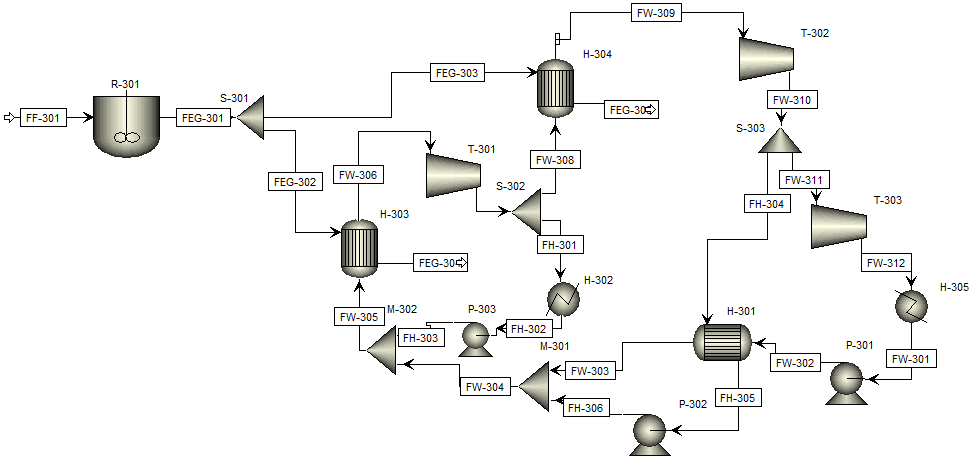
\includegraphics[width=.9\linewidth]{Block_300_-_Λέβητας_Καύσης_Λιγνίνης/2023-03-11_17-09-00_screenshot.png}
\caption{Block 300 στο Aspen}
\end{figure}

Εφόσον αυτό το block χρησιμοποιεί ένα κύκλο Rankine για ηλεκτροπαραγωγή (λόγω της τεράστιας περίσσειας θερμικής ενέργειας που έχει), τα ρεύματα του δεν θα ληφθούν υπόψην στην ολοκλήρωση της διεργασίας, αλλά όπου χρειάζεται βοηθητική θερμή παροχή θα υποθέτεται ότι είναι η παροχή FH-301 του διαγράμματος αυτού, η οποία είναι ατμός στα 40 bar και 364.8 \(^oC\) και η ποσότητα της θα είναι τέτοια ώστε να είναι αρκετή για όλα τα θερμά της διεργασίας.

\subsection{Block 400 - Παραγωγή Γλυκερόλης}
\label{sec:org84b88cc}
Στο block αυτό φαίνεται ο βιοαντιδραστήρας του μικροοργανισμού C. glycerinogenes ο οποίος χρησιμοποιείται για την παραγωγή γλυκερόλης. Ως τροφοδοσία χρησιμοποιείται ένα μίγμα υδατικού διαλύματος γλυκόζης μαζί με ουρία (πηγή αζώτου) και επαρκές οξυγόνο για την αερόβια καλλιέργεια. Επίσης στο feed υπάρχει και μικρή ποσότητα βιομάζας για να ξεκινήσει η αντίδραση.

\begin{figure}[htbp]
\centering
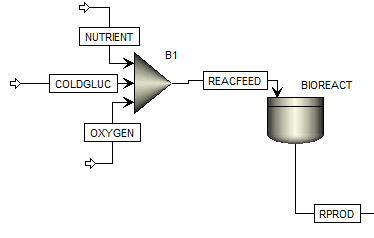
\includegraphics[width=.9\linewidth]{Block_400_-_Παραγωγή_Γλυκερόλης/2023-03-11_17-15-10_screenshot.png}
\caption{Block 400 στο Aspen}
\end{figure}

Στο block αυτό, όλα τα ρεύματα τροφοδοτούνται στους 30 \(^oC\) και αντιδρούν σε αντιδραστήρα σταθερής θερμοκρασίας. Άρα, δεν υπάρχει καμία μεταβολή στην θερμοκρασία των ρευμάτων και άρα κανένα θερμό ή ψυχρό ρεύμα να χρησιμοποιηθεί.

\subsection{Block 500 - Καθαρισμός Γλυκερόλης}
\label{sec:org9b19c14}
Το block αυτό είναι για τον διαχωρισμό των προιόντων του βιοαντιδραστήρα και την ανάκτηση της καθαρής εμπορεύσιμης γλυκερόλης. Τροφοδοσία του είναι το προιόν του block 400, δηλαδή τα προιόντα του βιοαντιδραστήρα μετά την πρώτη βαθμίδα θέρμανσης από την γλυκερόλη. Προιόν της διεργασίας είναι η καθαρή γλυκερόλη και δύο υδατικά κλάσματα τα οποία χρησιμοποιούνται για την θέρμανση.

\begin{figure}[htbp]
\centering
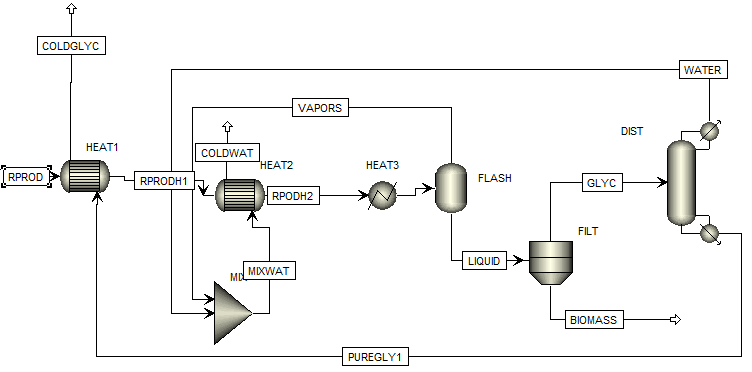
\includegraphics[width=.9\linewidth]{Block_500_-_Καθαρισμός_Γλυκερόλης/2023-03-11_17-17-18_screenshot.png}
\caption{Block 500 στο Aspen}
\end{figure}

Στο block αυτό υπάρχουν:
\begin{itemize}
\item Θέρμανση του προιόντος του βιοαντιδραστήρα μέχρι τους 140 \(^oC\) για flash και έπειτα απόσταξη (ψυχρό ρεύμα).
\item Παραγωγή 3 διαθέσιμων θερμών ρευμάτων, ένα την ατμώδη φάση του flash, ένα με σχεδόν καθαρό νερό από το απόσταγμα της αποστακτικής και ένα καθαρής γλυκερόλης.

Ο χαρακτηρισμός των ρευμάτων αυτών είναι
\end{itemize}
\begin{center}
\begin{tabular}{llrrrl}
Ρεύμα & Είδος & Τ\textsubscript{in} (C) & Τ\textsubscript{out} (C) & Παροχή (kmol/hr) & Σύσταση\\
\hline
RProd & Ψυχρό & 30 & 140 & 774.29 & Νερό 0.89\\
 &  &  &  &  & CO\textsubscript{2} 0.08\\
 &  &  &  &  & Γλυκερόλη 0.02\\
 &  &  &  &  & Άλλα 0.01\\
\hline
FlashVaps & Θερμό & 140 & 30 & 745.99 & Νερό 0.91\\
 &  &  &  &  & CO\textsubscript{2} 0.089\\
 &  &  &  &  & Άλλα 0.01\\
\hline
GlycWater & Θερμό & 144.4 & 30 & 9.82 & Νερό\\
\hline
PureGlycerol & Θερμό & 288.9 & 30 & 15.9 & Γλυκερόλη\\
\hline
\end{tabular}
\end{center}

Αξίζει να αναφερθεί πως ο χαρακτηρισμός άλλα αναφέρεται σε περίσσεια αντιδρώντων (ουρία, οξυγόνο), την παραγόμενη βιομάζα και τα παραπροιόντα της αντίδρασης (οξικό οξύ και αιθανόλη) τα οποία είναι σε αρκετά μικρές ποσότητες συγκριτικά με το νερό, το CO\textsubscript{2} και την γλυκερόλη. Στους υπολογισμούς της ενεργειακής ολοκλήρωσης θα αγνοηθούν.

\subsection{Block 600 - Παραγωγή Κυκλοπεντανόνης με την Φουρφουράλη ως Ενδιάμεσο}
\label{sec:org6f82726}
Το block αυτό είναι αυτό που αξιοποιεί την ημικυτταρινική φάση της βιομάζας όπως αυτή βγαίνει από το steam explosion στο block 100. Στο block αυτό παράγεται αρχικά ένα ενδιάμεσο προιόν, η φουρφουράλη, από την ξυλόζη ενώ αυτή οδηγείται σε έναν δεύτερο αντιδραστήρα, όπου με προσθήκη υδρογόνου, η φουρφουράλη μετατρέπεται σε κυκλοπεντανόνη, το τελικό μας προιόν.

\begin{figure}[htbp]
\centering
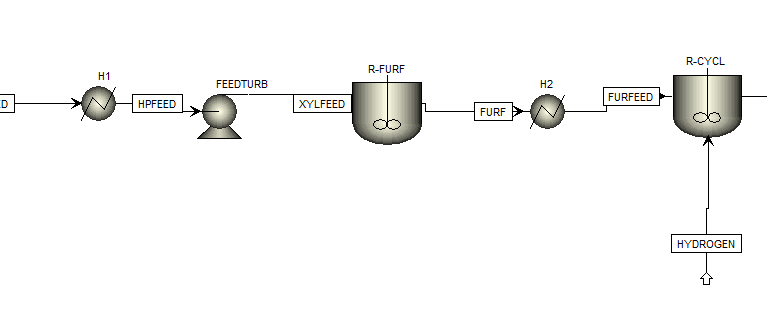
\includegraphics[width=.9\linewidth]{Block_600_-_Παραγωγή_Κυκλοπεντανόνης_με_την_Φουρφουράλη_ως_Ενδιάμεσο/2023-03-11_17-58-53_screenshot.png}
\caption{Block 600 στο Aspen}
\end{figure}

Στο block αυτό:
\begin{itemize}
\item Τροφοδοτείται αρχικά η ξυλόζη στους 232 \(^oC\) όπως βγήκε από την έκρηξη ατμού και θερμαίνεται μέχρι τους 243 \(^oC\) όπου λειτουργεί ο πρώτος αντιδραστήρας (ψυχρό ρεύμα)
\item Ψύχεται το προιόν της πρώτης αντίδρασης για να τροφοδοτηθεί στους 160 \(^oC\) στον 2ο αντιδραστήρα (θερμό ρεύμα).

Άρα τα διαθέσιμα ρεύματα είναι
\end{itemize}
\begin{table}[htbp]
\caption{Θερμά και Ψυχρά Ρεύματα στο Block 600}
\centering
\begin{tabular}{llrrrl}
Ρεύμα & Είδος & Τ\textsubscript{in} (C) & Τ\textsubscript{out} (C) & Παροχή (kmol/hr) & Σύσταση\\
\hline
XylFeed & Ψυχρό & 232 & 243 & 26.38 & Ξυλόζη\\
\hline
FurFeed & Θερμό & 243 & 160 & 105.52 & Νερό 0.75\\
 &  &  &  &  & Φουρφουράλη 0.25\\
\hline
\end{tabular}
\end{table}

\subsection{Block 700 - Καθαρισμός της Κυκλοπεντανόνης}
\label{sec:org9570105}
Το block αυτό έχει ως σκοπό τον καθαρισμό του προιόντος του block 600, δηλαδή του προιόντος του αντιδραστήρα της κυκλοπεντανόνης. Αυτό είναι μίγμα νερού-κυκλοπεντανόνης με μικρή περίσσεια φουρφουράλης και υδρογόνου από την αντίδραση. Προιόν της διεργασίας αυτής είναι η εμπορεύσιμη πλέον κυκλοπεντανόνη υψηλής καθαρότητας.

\begin{figure}[htbp]
\centering
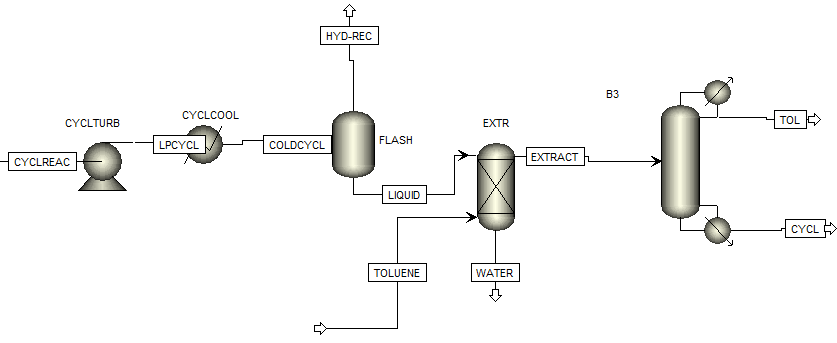
\includegraphics[width=.9\linewidth]{Block_700_-_Καθαρισμός_της_Κυκλοπεντανόνης/2023-03-17_18-13-36_screenshot.png}
\caption{Block 700 στο Aspen}
\end{figure}

Αρχικά το προιόν έρχεται σε θερμοκρασία και πίεση περιβάλλοντος. Έπειτα, περνάει ένα flash για να φύγει το αέριο υδρογόνο, μία εκχύλιση για να φύγει το νερό και τέλος μία απόσταξη για να διαχωριστεί η κυκλοπεντανόνη από τον διαλύτη (τολουόλιο). Το υδρογόνο και το νερό που απομακρύνονται είναι σε θερμοκρασία περιβάλλοντος άρα η θερμική τους εκμετάλλευση δεν έχει ιδιαίτερο νόημα.

\begin{table}[htbp]
\caption{Θερμά και Ψυχρά Ρεύματα στο Block 700}
\centering
\begin{tabular}{llrrrl}
Ρεύμα & Είδος & Τ\textsubscript{in} (C) & Τ\textsubscript{out} (C) & Παροχή (kmol/hr) & Σύσταση\\
\hline
CyclReac & Θερμό & 160 & 30 & 2132.66 & Κυκλοπεντανόνη 0.2\\
 &  &  &  &  & Νερό 0.79\\
 &  &  &  &  & Υδρογόνο 0.01\\
\hline
Cycl & Θερμό & 130 & 30 & 26 & Κυκλοπεντανόνη 0.98\\
 &  &  &  &  & Φουρφουράλη 0.015\\
 &  &  &  &  & Τολουόλιο 0.005\\
\hline
Tol & Θερμό & 50 & 30 & 51.02 & Τολουόλιο 0.98\\
 &  &  &  &  & Νερό 0.01\\
 &  &  &  &  & Κυκλοπεντανόνη 0.01\\
\hline
\end{tabular}
\end{table}

\subsection{Τελική εικόνα}
\label{sec:orgd89ec83}
Έχοντας δει όλα τα blocks ξεχωριστά, μπορούμε να φτιάξουμε τον συνολικό πίνακα ψυχρών και θερμών ρευμάτων ο οποίος είναι

\begin{longtable}{llrrrl}
\caption{Συνολικός Πίνακας Θερμών και Ψυχρών της διεργασίας}
\\
\hline
Ρεύμα & Είδος & Τ\textsubscript{in} (C) & Τ\textsubscript{out} (C) & Παροχή (kmol/hr) & Σύσταση\\
\hline
\endfirsthead
\multicolumn{6}{l}{Continued from previous page} \\
\hline

Ρεύμα & Είδος & Τ\textsubscript{in} (C) & Τ\textsubscript{out} (C) & Παροχή (kmol/hr) & Σύσταση \\

\hline
\endhead
\hline\multicolumn{6}{r}{Continued on next page} \\
\endfoot
\endlastfoot
\hline
FeedSteam & Ψυχρό & 20 & 232 & 633.22 & Νερό\\
\hline
Vapors & Θερμό & 232 & 30 & 905.27 & Νερό 0.92\\
 &  &  &  &  & CO\textsubscript{2} 0.08\\
\hline
CellLig & Θερμό & 232 & 80.65 & 84.76 & Κυτταρίνη 0.5\\
 &  &  &  &  & Λιγνίνη 0.5\\
\hline
NaOH & Ψυχρό & 20 & 80.65 & 80.37 & Νερό\\
\hline
Bleach & Ψυχρό & 20 & 69.9 & 55.62 & Νερό 99.5\\
 &  &  &  &  & Χλωρίνη 0.05\\
\hline
Cellulose & Θέρμο & 80.65 & 69.9 & 54.32 & Κυτταρίνη 0.78\\
 &  &  &  &  & Λιγνίνη 0.22\\
\hline
PureCell & Θερμό & 61.97 & 49.75 & 42.55 & Κυτταρίνη\\
\hline
SachWater & Ψυχρό & 20 & 49.75 & 715 & Νερό\\
\hline
Glucose & Θερμό & 50 & 30 & 669.45 & Νερό 0.97\\
 &  &  &  &  & Γλυκόζη 0.03\\
\hline
RProd & Ψυχρό & 30 & 140 & 774.29 & Νερό 0.89\\
 &  &  &  &  & CO\textsubscript{2} 0.08\\
 &  &  &  &  & Γλυκερόλη 0.02\\
 &  &  &  &  & Άλλα 0.01\\
\hline
FlashVaps & Θερμό & 140 & 30 & 745.99 & Νερό 0.91\\
 &  &  &  &  & CO\textsubscript{2} 0.089\\
 &  &  &  &  & Άλλα 0.01\\
\hline
GlycWater & Θερμό & 144.4 & 30 & 9.82 & Νερό\\
\hline
PureGlycerol & Θερμό & 288.9 & 30 & 15.9 & Γλυκερόλη\\
\hline
XylFeed & Ψυχρό & 232 & 243 & 26.38 & Ξυλόζη\\
\hline
FurFeed & Θερμό & 243 & 160 & 105.52 & Νερό 0.75\\
 &  &  &  &  & Φουρφουράλη 0.25\\
\hline
CyclReac & Θερμό & 160 & 30 & 2132.66 & Κυκλοπεντανόνη 0.2\\
 &  &  &  &  & Νερό 0.79\\
 &  &  &  &  & Υδρογόνο 0.01\\
\hline
Cycl & Θερμό & 130 & 30 & 26 & Κυκλοπεντανόνη 0.98\\
 &  &  &  &  & Φουρφουράλη 0.015\\
 &  &  &  &  & Τολουόλιο 0.005\\
\hline
Tol & Θερμό & 50 & 30 & 51.02 & Τολουόλιο 0.98\\
 &  &  &  &  & Νερό 0.01\\
 &  &  &  &  & Κυκλοπεντανόνη 0.01\\
\hline
\end{longtable}

Με αυτά τα δεδομένα μπορούν να υπολογιστούν οι ειδικές θερμοχωρητικότητες για όλα τα ρεύματα και έπειτα και οι θερμοχωρητικότητες. Αρχικά, παρατίθεται ένας πίνακας με την θερμοχωρητικότητα κάθε ουσίας που μας ενδιαφέρει
\begin{table}[htbp]
\caption{Θερμοχωρητικότητες ουσιών}
\centering
\begin{tabular}{lr}
Ουσία & Cp (J/mol K)\\
\hline
Νερό & 75.38\\
Κυτταρίνη & 89.63\\
Λιγνίνη & 90.98\\
Γλυκόζη & 225\\
Γλυκερόλη & 225.4\\
CO\textsubscript{2} & 37.35\\
Ξυλόζη & 178.1\\
Φουρφουράλη & 159.5\\
Κυκλοπεντανόνη & 112.18\\
Υδρογόνο & 14.5\\
Τολουόλιο & 158.4\\
\hline
\end{tabular}
\end{table}

και από αυτά υπολογίζονται οι ειδικές θερμοχωρητικότητες και οι θερμοχωρητικότητες των ρευμάτων
\begin{longtable}{lrrr}
\caption{Θερμοχωρητικότητες ρευμάτων}
\\
Ρεύμα & Παροχή (kmol/h) & Cp (J/mol K) & CP (MJ/h K)\\
\hline
\endfirsthead
\multicolumn{4}{l}{Continued from previous page} \\
\hline

Ρεύμα & Παροχή (kmol/h) & Cp (J/mol K) & CP (MJ/h K) \\

\hline
\endhead
\hline\multicolumn{4}{r}{Continued on next page} \\
\endfoot
\endlastfoot
\hline
FeedSteam & 633.22 & 75.38 & 47.732124\\
StExpVapors & 905.27 & 72.34 & 65.487232\\
CellLig & 84.76 & 90.31 & 7.6546756\\
NaOH & 80.37 & 75.38 & 6.0582906\\
Bleach & 55.62 & 75.38 & 4.1926356\\
Cellulose & 54.32 & 89.93 & 4.8849976\\
PureCell & 42.55 & 89.63 & 3.8137565\\
SachWater & 715 & 75.38 & 53.8967\\
Glucose & 669.45 & 79.87 & 53.468972\\
RProd & 774.29 & 74.58 & 57.746548\\
FlashVapors & 745.99 & 71.96 & 53.681440\\
GlycWater & 9.82 & 75.38 & 0.7402316\\
PureGlyc & 15.9 & 225.4 & 3.58386\\
XylFeed & 26.38 & 178.1 & 4.698278\\
FurFeed & 105.52 & 96.41 & 10.173183\\
CyclReac & 24.61 & 112.71 & 2.7737931\\
CyclWater & 106.9 & 76.12 & 8.137228\\
\end{longtable}

Επίσης, μπορεί να κατασκευαστεί και ο πίνακας των ανηγμένων θερμοκρασιών του συστήματος
\begin{table}[htbp]
\caption{Πίνακας ανηγμένων θερμοκρασιών}
\centering
\begin{tabular}{llrr}
Ρεύμα & Είδος & Τ\textsubscript{in} (C) & T\textsubscript{out} (C)\\
\hline
FeedSteam & Ψυχρό & 25 & 237\\
StExpVapors & Θερμό & 227 & 25\\
CellLig & Θερμό & 227 & 75.65\\
NaOH & Ψυχρό & 25 & 85.65\\
Bleach & Ψυχρό & 25 & 74.9\\
Cellulose & Θερμό & 75.65 & 64.9\\
PureCell & Θερμό & 56.97 & 44.75\\
SachWater & Ψυχρό & 25 & 54.75\\
Glucose & Θερμό & 45 & 25\\
RProd & Ψυχρό & 35 & 145\\
FlashVaps & Θερμό & 135 & 25\\
GlycWater & Θερμό & 139.4 & 25\\
PureGlycerol & Θερμό & 283.9 & 25\\
XylFeed & Ψυχρό & 237 & 248\\
FurFeed & Θερμό & 238 & 155\\
Cyclo & Θερμό & 262.8 & 25\\
CyclWater & Θερμό & 196.5 & 25\\
\end{tabular}
\end{table}

Με βάση τους δύο αυτούς πίνακες μπορεί να γίνει η ενεργειακή ολοκλήρωση

\section{Υπολογισμοί Ενεργειακής Ολοκλήρωσης}
\label{sec:org10a0885}
Αρχικά, φτιάχνουμε τον χρήσιμο αυτό πίνακα.

\begin{longtable}{rrrrrrr}
\caption{Χαρακτηρισμός των "ψευδο"-ρευμάτων του ενεργειακού καταρράκτη}
\\
Τ\textsubscript{1} & T\textsubscript{2} & ΔΤ & CPc & CPh & CP & ΔΗ\\
\hline
\endfirsthead
\multicolumn{7}{l}{Continued from previous page} \\
\hline

Τ\textsubscript{1} & T\textsubscript{2} & ΔΤ & CPc & CPh & CP & ΔΗ \\

\hline
\endhead
\hline\multicolumn{7}{r}{Continued on next page} \\
\endfoot
\endlastfoot
\hline
283.9 & 248 & 35.9 & 0 & 3.584 & -3.584 & -128.6656\\
248 & 238 & 10 & 4.698 & 3.584 & 1.114 & 11.14\\
238 & 237 & 1 & 4.698 & 13.757 & -9.059 & -9.059\\
237 & 227 & 10 & 47.732 & 13.757 & 33.975 & 339.75\\
227 & 155 & 72 & 47.732 & 83.315 & -35.583 & -2561.976\\
155 & 145 & 10 & 47.732 & 91.792 & -44.06 & -440.6\\
145 & 139.4 & 5.6 & 105.479 & 91.792 & 13.687 & 76.6472\\
139.4 & 135 & 4.4 & 105.479 & 92.532 & 12.947 & 56.9668\\
135 & 125 & 10 & 105.479 & 161.279 & -55.8 & -558.\\
125 & 85.65 & 39.35 & 105.479 & 150.889 & -45.41 & -1786.8835\\
85.65 & 75.65 & 10. & 111.537 & 150.889 & -39.352 & -393.52\\
75.65 & 74.9 & 0.75 & 111.537 & 148.119 & -36.582 & -27.4365\\
74.9 & 64.9 & 10. & 115.730 & 148.119 & -32.389 & -323.89\\
64.9 & 56.97 & 7.93 & 115.730 & 143.233 & -27.503 & -218.09879\\
56.97 & 54.75 & 2.22 & 115.730 & 147.048 & -31.318 & -69.52596\\
54.75 & 45 & 9.75 & 169.627 & 147.048 & 22.579 & 220.14525\\
45 & 35 & 10 & 169.627 & 208.023 & -38.396 & -383.96\\
35 & 25 & 10 & 111.880 & 208.023 & -96.143 & -961.43\\
\end{longtable}

ο οποίος θα ειναι και το κύριο εργαλείο που θα χρησιμοποιήσουμε για την ολοκλήρωση.

Με βάση αυτό, μπορεί να φτιαχθεί και το μεγάλο σύνθετο γράφημα.

Από τον παρακάτω πίνακα, αν dH ο πίνακας των ενθαλπιών, μπορεί να υπολογιστεί η ενεργειακή στάθμη για το μεγάλο σύνθετο γράφημα από τον κώδικα
\texttt{cumdH = -min(cumsum(-dH)) + cumsum(-dH)}
από τα οποία προκύπτει ο πίνακας

\begin{longtable}{rr}
\caption{Δεδομένα για τον ενεργειακό καταρράκτη}
\\
Cumulative  Dh & T\\
\hline
\endfirsthead
\multicolumn{2}{l}{Continued from previous page} \\
\hline

Cumulative  Dh & T \\

\hline
\endhead
\hline\multicolumn{2}{r}{Continued on next page} \\
\endfoot
\endlastfoot
\hline
213.165 & 283.9\\
341.831 & 248\\
330.691 & 238\\
339.750 & 237\\
0 & 227\\
2561.976 & 155\\
3002.576 & 145\\
2925.928 & 139.4\\
2868.962 & 135\\
3426.962 & 125\\
5213.845 & 85.65\\
5607.365 & 75.65\\
5634.802 & 74.9\\
5958.692 & 64.9\\
6176.790 & 56.97\\
6246.316 & 54.75\\
6026.171 & 45\\
6410.131 & 35\\
7371.561 & 25\\
\end{longtable}

\begin{figure}[htbp]
\centering
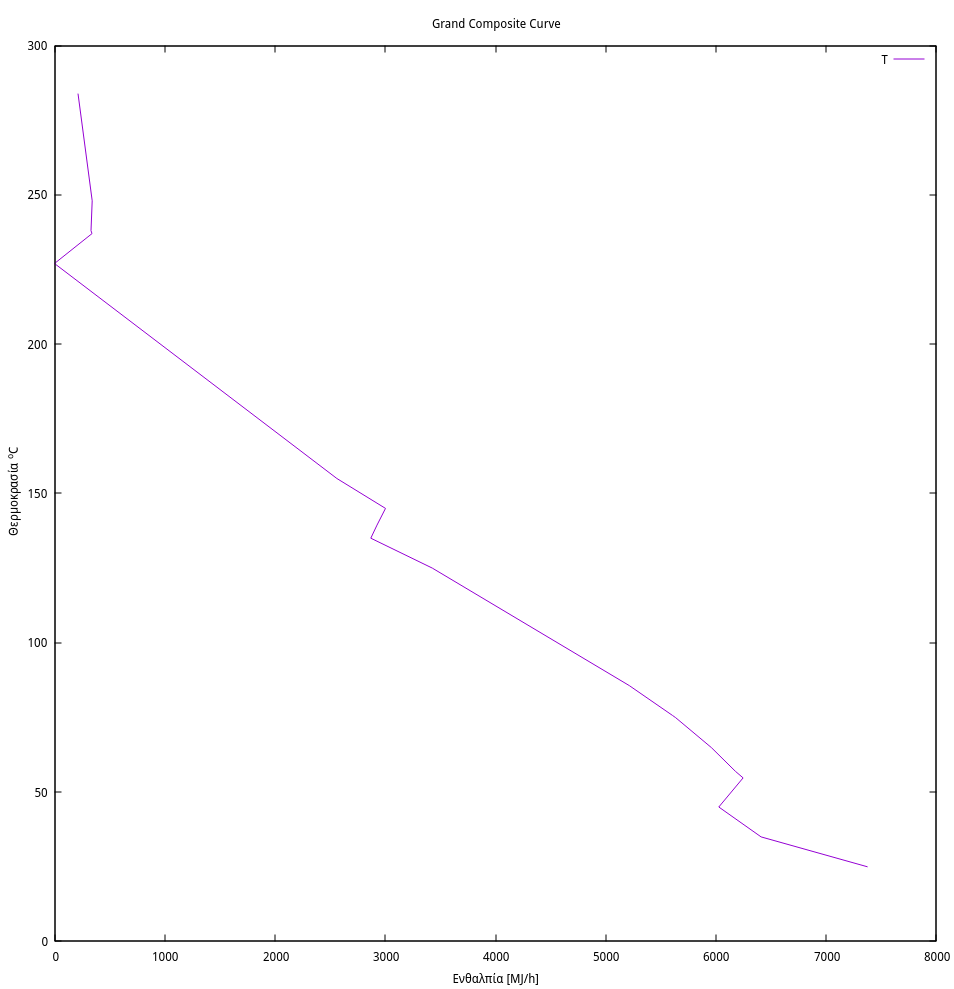
\includegraphics[width=.9\linewidth]{Diagrams/grand_composite_curve.png}
\caption{Μεγάλο Σύνθετο Γράφημα}
\end{figure}

Με τα ρεύματα αυτά ως έχουν, προκύπτει ότι απαιτείται μία μεγάλη ποσότητα ψυχρής παροχής και μικρή ποσότητα θερμής. Αυτό είναι ανεπιθύμητο επειδή η μονάδα έχει διαθέσιμη θερμή παροχή δωρεάν ενώ το ίδιο δεν ισχύει για την ψυχρή παροχή. Βέβαια, πολύ από αυτήν την απαίτηση οφείλεται στην εκμετάλλευση του θερμικού περιεχομένου των προιόντων τα οποία δεν είναι ανάγκη να ψυχθούν και τα εκμεταλλευόμαστε μόνο αν βοηθάνε.

\subsection{Εναλλακτικά σενάρια ολοκλήρωσης}
\label{sec:orgc6057a7}

Τα δύο σημαντικότερα θερμά ρεύματα που συνεισφέρουν σε αυτό το ανεπιθύμητο αποτέλεσμα είναι οι ατμοί της έκρηξης ατμού (οι οποίοι είναι σε πολύ υψηλή θερμοκρασία και είναι αρκετά μεγάλη ποσότητα) και οι ατμοί του flash στον καθαρισμό της γλυκερόλης που είναι επίσης μεγάλη ποσότητα νερού στην ατμώδη φάση. Αν δεν χρησιμοποιηθεί τίποτα από τα δύο, το αποτέλεσμα θα είναι πως αντί για πολύ ψυχρή παροχή, χρειαζόμαστε πολύ θερμή παροχή. Έστω ότι χρησιμοποιούμε μόνο τους ατμούς του flash και όχι αυτούς της έκρηξης ατμού (οι οποίοι έχουν και μεγαλύτερο θερμοκρασιακό εύρος και μεγαλύτερη θερμοχωρητικότητα).

\begin{table}[htbp]
\caption{Καταρράκτης χωρίς steam explosion vapors}
\centering
\begin{tabular}{rrrrrrr}
Τ\textsubscript{1} & T\textsubscript{2} & ΔΤ & CPc & CPh & CP & ΔΗ\\
\hline
283.9 & 248 & 35.9 & 0 & 3.584 & -3.584 & -128.6656\\
248 & 238 & 10 & 4.698 & 3.584 & 1.114 & 11.14\\
238 & 237 & 1 & 4.698 & 13.757 & -9.059 & -9.059\\
237 & 227 & 10 & 47.732 & 13.757 & 33.975 & 339.75\\
227 & 155 & 72 & 47.732 & 17.828 & 29.904 & 2153.088\\
155 & 145 & 10 & 47.732 & 26.305 & 21.427 & 214.27\\
145 & 139.4 & 5.6 & 105.479 & 26.305 & 79.174 & 443.3744\\
139.4 & 135 & 4.4 & 105.479 & 27.045 & 78.434 & 345.1096\\
135 & 125 & 10 & 105.479 & 95.792 & 9.687 & 96.87\\
125 & 85.65 & 39.35 & 105.479 & 85.402 & 20.077 & 790.02995\\
85.65 & 75.65 & 10. & 111.537 & 85.402 & 26.135 & 261.35\\
75.65 & 74.9 & 0.75 & 111.537 & 82.632 & 28.905 & 21.67875\\
74.9 & 64.9 & 10. & 115.730 & 82.632 & 33.098 & 330.98\\
64.9 & 56.97 & 7.93 & 115.730 & 77.746 & 37.984 & 301.21312\\
56.97 & 54.75 & 2.22 & 115.730 & 81.561 & 34.169 & 75.85518\\
54.75 & 45 & 9.75 & 169.627 & 81.561 & 88.066 & 858.6435\\
45 & 35 & 10 & 169.627 & 142.536 & 27.091 & 270.91\\
35 & 25 & 10 & 111.880 & 142.536 & -30.656 & -306.56\\
\end{tabular}
\end{table}

\begin{longtable}{rr}
\caption{Δεδομένα για τον ενεργειακό καταρράκτη}
\\
Cumulative  Dh & T\\
\hline
\endfirsthead
\multicolumn{2}{l}{Continued from previous page} \\
\hline

Cumulative  Dh & T \\

\hline
\endhead
\hline\multicolumn{2}{r}{Continued on next page} \\
\endfoot
\endlastfoot
\hline
6376.537 & 283.9\\
6505.203 & 248\\
6494.063 & 238\\
6503.122 & 237\\
6163.372 & 227\\
4010.284 & 155\\
3796.014 & 145\\
3352.640 & 139.4\\
3007.530 & 135\\
2910.660 & 125\\
2120.630 & 85.65\\
1859.280 & 75.65\\
1837.601 & 74.9\\
1506.621 & 64.9\\
1205.408 & 56.97\\
1129.553 & 54.75\\
270.91 & 45\\
0 & 35\\
306.56 & 25\\
\end{longtable}


Το ΜΣΓ της περίπτωσης αυτής φαίνεται στην επόμενη σελίδα.

Με βάση το αποτέλεσμα αυτό, θεωρείται ότι υπάρχει περιθώριο να εκμεταλλευτούμε το θερμό ρεύμα που παραλείψαμε (καθώς υπάρχει μία σχετικά μεγάλη απαίτηση σε θερμό), αλλά δεν υπάρχει λόγος να ψυχθεί αυτό μέχρι χαμηλή θερμοκρασία επειδή όσο περισσότερο ψύχεται, τόσο περισσότερη ψυχρή παροχή θα θέλουμε. Από τους παραπάνω υπολογισμούς, βλέπουμε ότι η συνολική θερμοχωρητικότητα των θερμών είναι χαμηλή μέχρι τους 135 \(^oC\) και μετά, που αρχίζουν να ψύχονται οι ατμοί του flash από τον καθαρισμό της γλυκερόλης, οι οποίοι έχουν υψηλή θερμοχωρητικότητα, υπάρχει αρκετή θερμή παροχή. Άρα, είναι αρκετά πιθανό η ψύξη των ατμών του steam explosion μέχρι τους 135 \(^oC\) στο ΜΣΓ (δηλαδή 140 \(^oC\)) να είναι βοηθητική, μειώνοντας σημαντικά την απαίτηση σε θερμή παροχή χωρίς να αυξάνει πολύ την απαίτηση σε ψυχρή βοηθητική παροχή.

\begin{longtable}{rrrrrrr}
\caption{Καταρράκτης με μερική ψύξη των ατμών του steam explosion}
\\
Τ\textsubscript{1} & T\textsubscript{2} & ΔΤ & CPc & CPh & CP & ΔΗ\\
\hline
\endfirsthead
\multicolumn{7}{l}{Continued from previous page} \\
\hline

Τ\textsubscript{1} & T\textsubscript{2} & ΔΤ & CPc & CPh & CP & ΔΗ \\

\hline
\endhead
\hline\multicolumn{7}{r}{Continued on next page} \\
\endfoot
\endlastfoot
\hline
283.9 & 248 & 35.9 & 0 & 3.584 & -3.584 & -128.6656\\
248 & 238 & 10 & 4.698 & 3.584 & 1.114 & 11.14\\
238 & 237 & 1 & 4.698 & 13.757 & -9.059 & -9.059\\
237 & 227 & 10 & 47.732 & 13.757 & 33.975 & 339.75\\
227 & 155 & 72 & 47.732 & 83.315 & -35.583 & -2561.976\\
155 & 145 & 10 & 47.732 & 91.792 & -44.06 & -440.6\\
145 & 139.4 & 5.6 & 105.479 & 91.792 & 13.687 & 76.6472\\
139.4 & 135 & 4.4 & 105.479 & 92.532 & 12.947 & 56.9668\\
135 & 125 & 10 & 105.479 & 95.792 & 9.687 & 96.87\\
125 & 85.65 & 39.35 & 105.479 & 85.402 & 20.077 & 790.02995\\
85.65 & 75.65 & 10. & 111.537 & 85.402 & 26.135 & 261.35\\
75.65 & 74.9 & 0.75 & 111.537 & 82.632 & 28.905 & 21.67875\\
74.9 & 64.9 & 10. & 115.730 & 82.632 & 33.098 & 330.98\\
64.9 & 56.97 & 7.93 & 115.730 & 77.746 & 37.984 & 301.21312\\
56.97 & 54.75 & 2.22 & 115.730 & 81.561 & 34.169 & 75.85518\\
54.75 & 45 & 9.75 & 169.627 & 81.561 & 88.066 & 858.6435\\
45 & 35 & 10 & 169.627 & 142.536 & 27.091 & 270.91\\
35 & 25 & 10 & 111.880 & 142.536 & -30.656 & -306.56\\
\end{longtable}

\pagebreak

\begin{figure}[htbp]
\centering
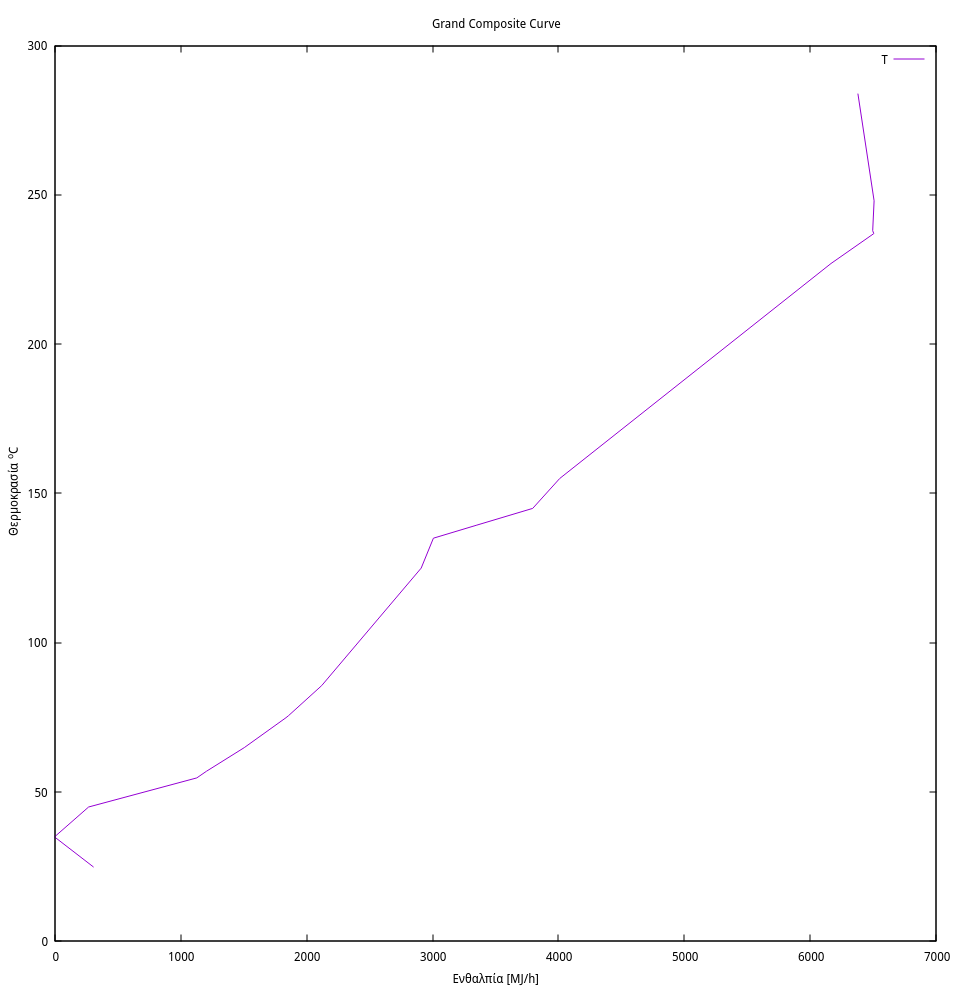
\includegraphics[width=400px]{Diagrams/grand_composite_curve_2.png}
\caption{Μεγάλο Σύνθετο Γράφημα χωρίς τους ατμούς της έκρηξης ατμού}
\end{figure}

\begin{table}[htbp]
\caption{Δεδομένα για τον ενεργειακό καταρράκτη}
\centering
\begin{tabular}{rr}
Cumulative  Dh & T\\
\hline
351.734 & 283.9\\
480.399 & 248\\
469.259 & 238\\
478.318 & 237\\
138.568 & 227\\
2700.544 & 155\\
3141.144 & 145\\
3064.497 & 139.4\\
3007.530 & 135\\
2910.660 & 125\\
2120.630 & 85.65\\
1859.280 & 75.65\\
1837.601 & 74.9\\
1506.621 & 64.9\\
1205.408 & 56.97\\
1129.553 & 54.75\\
270.91 & 45\\
0 & 35\\
306.56 & 25\\
\end{tabular}
\end{table}

\begin{figure}[htbp]
\centering
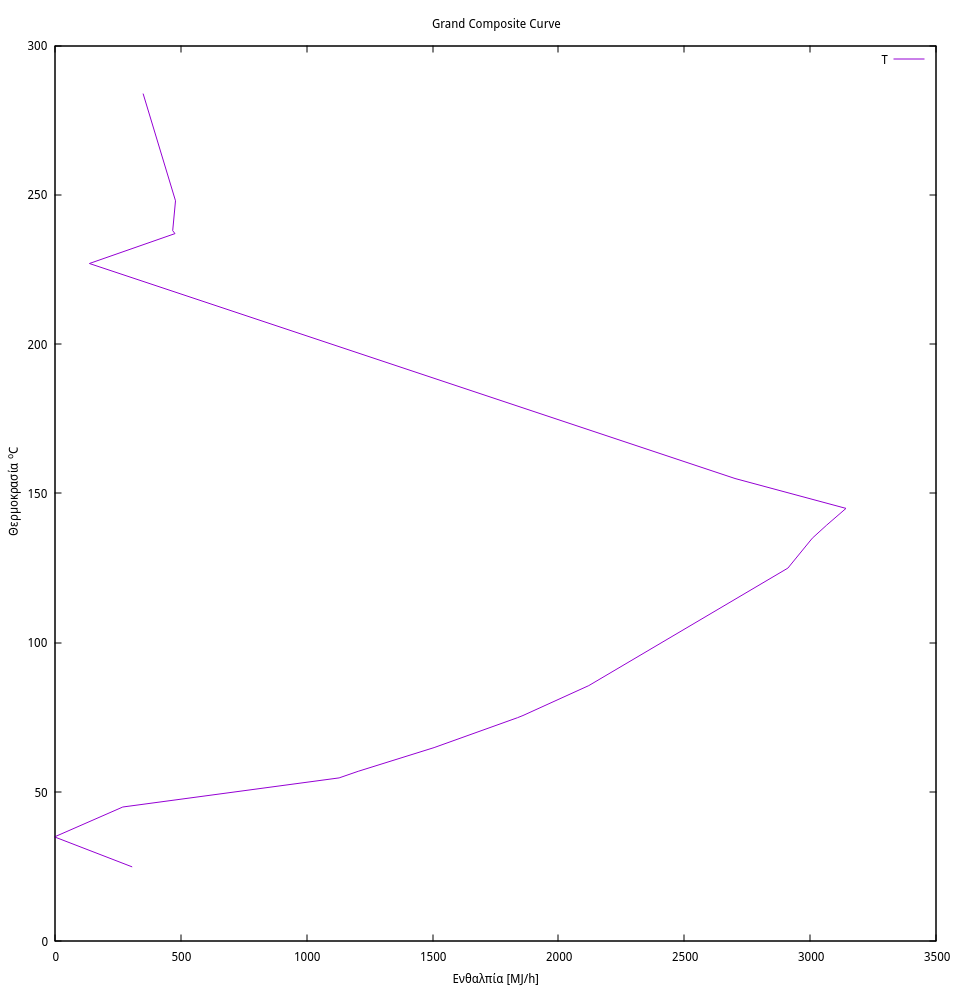
\includegraphics[width=400px]{Diagrams/grand_composite_curve_3.png}
\caption{Μεγάλο Σύνθετο Γράφημα με μερική ψύξη των ατμών της έκρηξης ατμού}
\end{figure}

\pagebreak

\subsection{Συμπεράσματα}
\label{sec:orgfcc1b93}
Συμπέρασμα ότι με την ενεργειακή ολοκλήρωση αυτή, η οποία θεωρείται και η καλύτερη, οι ενεργειακές απαιτήσεις της διεργασίας γίνονται

Απαίτηση σε ψυχρή παροχή 306.56 MJ/h σε θερμοκρασία κάτω από 25 \(^oC\) στο ΜΣΓ (δηλαδή κάτω από 20 \(^oC\), άρα στους 15 \(^oC\) πχ).

Απαίτηση σε θερμή παροχή: 351.73 MJ/h. Αν εκμεταλλευτούμε την μικρή τσέπη που δημιουργείται στο πάνω μέρος του ΜΣΓ, τότε η θερμή παροχή πρέπει να διατίθεται τουλάχιστον στους 235 \(^oC\) σε αυτό (δηλαδή τουλάχιστον 240 \(^oC\) αν χρησιμοποιούμε την πραγματική θερμοκρασία), αλλιώς πρέπει να διατίθεται στους 284 \(^oC\) τουλάχιστον. 

Επίσης, πέρα από αυτήν την ενεργειακή τσέπη η οποία έχει δημιουργηθεί και επιτρέπει ο ατμός που παράγεται να είναι σε χαμηλότερη ενεργειακή στάθμη, υπάρχει και άλλη μία, η οποία είναι πάρα πολύ σημαντικής έκτασης και επιτρέπει την πλήρη ενεργειακή αυτονομία όλων των ρευμάτων από 227 \(^oC\) μέχρι λίγο πάνω από 45 \(^oC\).

Επίσης, αξίζει να σημειωθεί πως ο κόμβος ανάσχεσης είναι το δεύτερο σημείο του γραφήματος με το πρώτο να είναι πολύ μικρό. Άρα, οι περιοχές μέσα και κάτω από τον κόμβο ανάσχεσης είναι πολύ μικρές. Αυτό μπορεί να δημιουργήσει προβλήματα εάν θέλουμε να ολοκληρώσουμε μία αντλία θερμότητας (μέσα από τον κόμβο ανάσχεσης) ή έναν ενδόθερμο αντιδραστήρα (κάτω από τον κόμβο ανάσχεσης).

\subsubsection{Σχόλια για την ολοκλήρωση διάφορων κομματιών}
\label{sec:orgf13442a}
\begin{enumerate}
\item Αντιδραστήρας παραγωγής γλυκερόλης
\label{sec:orgba7b0c4}
Ο αντιδραστήρας λειτουργεί στους 30 βαθμούς κελσίου και είναι εξώθερμος. Στο μεγάλο σύνθετο γράφημα θα έμπαινε στους 25 \(^oC\) το οποίο είναι κάτω από τον κόμβο ανάσχεσης κατά 10. Λόγω της πολύ στενής θερμοκρασιακής περιοχής στην οποία μπορεί να διεξαχθεί η αντίδραση, θεωρούμε πως δεν αξίζει να μελετηθεί ένα σενάριο ολοκλήρωσης του αντιδραστήρα αυτού με την υπόλοιπη διεργασία (όπου θα έπρεπε η θερμοκρασία λειτουργίας να αυξηθεί κατά 10 τουλάχιστον βαθμούς). Ακόμη όμως και να γινόταν, η απαίτηση σε ψύξη είναι υψηλή (12901.5 MJ/hr) και με την υπάρχουσα διεργασία και ολοκλήρωση, δεν περισσεύει πουθενά τόση ψυχρή παροχή.
\item Αποστακτική στήλη γλυκερόλης
\label{sec:orgc1fc247}
Ο αναβραστήρας της στήλης λειτουργεί στους 293 \(^oC\) στο ΜΣΓ και έχει απαίτηση θερμότητας στους 1105.44 MJ/hr. Αυτό υπερβαίνει τις θερμοκρασίες καθώς και τις ενθαλπίες που υπάρχουν στο διάγραμμα. Άρα, η ολοκλήρωση όλης της στήλης με το υπόλοιπο διάγραμμα ροής είναι ανέφικτη. Όμως, ο συμπηκνωτήρας της στήλης λειτουργεί στους 145 \(^oC\) (140 \(^oC\) στο ΜΣΓ). Στο σημείο αυτό είναι η μεγάλη ενεργειακή τσέπη του ΜΣΓ, άρα η ολοκλήρωση είναι αρκετά εύκολη. Επίσης, η απαίτηση σε ψύξη είναι σχετικά μικρή (149.49 MJ/hr) άρα ο συμπηκνωτήρας αυτός θα μπορούσε να ολοκληρωθεί ως εναλλάκτης αλλά όχι ως ολόκληρη αποστακτική.
\item Αντιδραστήρας παραγωγής φουρφουράλης
\label{sec:orgb3f7918}
Θερμοκρασία λειτουργίας οι 242 \(^oC\), ή 237 \(^oC\) στο μεγάλο σύνθετο γράφημα. Ο αντιδραστήρας είναι εξώθερμος, άρα μπορεί να γίνει σωστή ολοκλήρωση. Καθώς είναι αρκετά ψηλά στο γράφημα, υπάρχουν σίγουρα ρεύματα πιο ψυχρά από αυτό για να το ψύξουν. Επίσης, η απαίτηση του σε ψύξη είναι αρκετά χαμηλή (13.35 MJ/hr) άρα είναι αρκετά εύκολο να χωρέσει.
\item Αντιδραστήρας παραγωγής κυκλοπεντανόνης
\label{sec:org9b44a69}
Ο αντιδραστήρας αυτός λειτουργεί στους 160 \(^oC\) και είναι εξώθερμος (ως αντίδραση υδρογόνωσης). Στο σημείο αυτό υπάρχει διαθέσιμη θερμική ενέργεια λόγω της ενεργειακής τσέπης (της τάξης των 2500 MJ/hr). Βέβαια, ο θερμοτονισμός της αντίδρασης είναι μίας τάξης μεγέθους πάνω από την απαίτηση αυτή άρα δεν μπορεί να καλυφθεί η ανάγκη από τα υπάρχοντα ρεύματα.
\item Αποστακτική στήλη κυκλοπεντανόνης
\label{sec:org08af8eb}
Οι θερμικές απαιτήσεις της στήλης υπερβαίνουν την διαθέσιμη θερμότητα της διεργασίας άρα στην παρούσα φάση δεν μπορεί να ολοκληρωθεί. Η απαίτηση σε ψυχρό είναι 8999.76 MJ/hr, η οποία μπορεί να ικανοποιηθεί με νερό ψύξης ενώ αυτή σε θερμό είναι 9543.12 MJ/hr η οποία πρέπει να είναι ατμός σε θερμοκρασία τουλάχιστον 140 \(^oC\). Εφόσον αυτή θα παραχθεί από το κύκλο Rankine, είναι εύκολο να ρυθμιστεί κατάλληλα.
\item Αντιδραστήρας σακχαροποίησης
\label{sec:orgb1d0545}
Ο αντιδραστήρας λειτουργεί στους 50 \(^oC\) και είναι ενδόθερμος. Είναι πάνω από τον κόμβο ανάσχεσης, αλλά μέσα σε μία σχετικά μεγάλη ενεργειακή τσέπη. Στο σημείο αυτό της τσέπης υπάρχει διαθέσιμη περίπου 1000 MJ/hr θερμών παροχών και η απαίτηση του αντιδραστήρα είναι (393.63 MJ/hr) άρα η ολοκλήρωση θεωρείται εφικτή.
\end{enumerate}

\subsubsection{Αλλαγές στο ΜΣΓ}
\label{sec:org23f3851}
Για την αποστακτική της γλυκερόλης, αναφέρθηκε πως μπορεί να ολοκληρωθεί ως εναλλάκτης ο συμπυκνωτήρας χωρίς να ολοκληρώσουμε όλη την στήλη λόγω ανεπάρκειας ενέργειας. Άρα, στους 140 \(^oC\) μπορούμε να πούμε πως υπάρχει ένα επιπλέον θερμό ρεύμα το οποίο έχει ενθαλπία 149.49 MJ/hr. Άρα, μπορεί η περιοχή από τους 145 μέχρι τους 139.4 να μειώσει την ενθαλπία της κατά αυτόν τον αριθμό. Η ολοκλήρωση αυτή μετακινεί τον κόμβο ανάσχεσης αρκετά πιο ψηλά στο ΜΣΓ (227 \(^oC\)) και κάνει τον παλιό κόμβο ανάσχεσης να είναι στα 11 περίπου MJ/hr αντί για 0. Η ολοκλήρωση του αντιδραστήρα οδηγεί σε απαίτηση σε θερμή παροχή η οποία είναι περίπου το 0.6 της αρχικής και σε ελάχιστη αύξηση της απαίτησης σε ψυχρή παροχή, άρα είναι όντως ένα επιθυμητό σενάριο ολοκλήρωσης.

Ομοίως, ο αντιδραστήρας της φουρφουράλης είναι ένας εξώθερμος αντιδραστήρας που μπορεί να λειτουργήσει ως επιπλέον θερμό ρεύμα για την διεργασία με θερμότητα 13.35 MJ/hr στους 237 (θα προστεθεί στο interval 237->227). Αν προσθέσουμε και το ρεύμα αυτό στην προηγούμενη ολοκλήρωση, παρατηρούμε μία μικρή μείωση της απαίτησης σε θερμή παροχή (213.2->199.8) καθώς και μικρή αύξηση της ενεργειακής τσέπης πάνω από τον κόμβο ανάσχεσης. Άρα, έχει θετική επίδραση παρότι αρκετά μικρότερη από την παραπάνω.

Τέλος, ο τρίτος αντιδραστήρας που αναφέρθηκε ότι μπορεί να ολοκληρωθεί είναι ο αντιδραστήρας της σακχαροποίησης της κυτταρίνης ο οποίος όμως είναι ενδόθερμος, άρα λειτουργεί ως ένα ψυχρό ρεύμα στους 55 \(^oC\) το οποίο προσθέτει 393.63 MJ/hr στο interval 56.97->54.75. Η ολοκλήρωση αυτή οδηγεί σε μία αρκετά μικρή μείωση της ψυχρής παροχής αλλά επίσης προκαλεί σχεδόν τριπλασιασμό της απαίτησης σε θερμή παροχή. Συμπέρασμα πως δεν αξίζει να γίνει μία τέτοια ολοκλήρωση όπως και οι υπόλοιπες ολοκληρώσεις του ΜΣΓ.

Παρακάτω παρατίθεται και το ΜΣΓ στο οποίο έχουν γίνει οι δύο αυτές προσθήκες.
\begin{table}[htbp]
\caption{Δεδομένα για τον ενεργειακό καταρράκτη}
\centering
\begin{tabular}{rr}
Cumulative  Dh & T\\
\hline
199.815 & 283.9\\
328.481 & 248\\
317.341 & 238\\
326.4 & 237\\
0 & 227\\
2561.976 & 155\\
3002.576 & 145\\
3075.419 & 139.4\\
3018.452 & 135\\
2921.582 & 125\\
2131.552 & 85.65\\
1870.202 & 75.65\\
1848.523 & 74.9\\
1517.543 & 64.9\\
1216.330 & 56.97\\
1140.475 & 54.75\\
281.831 & 45\\
10.921 & 35\\
317.481 & 25\\
\end{tabular}
\end{table}

\begin{figure}[htbp]
\centering
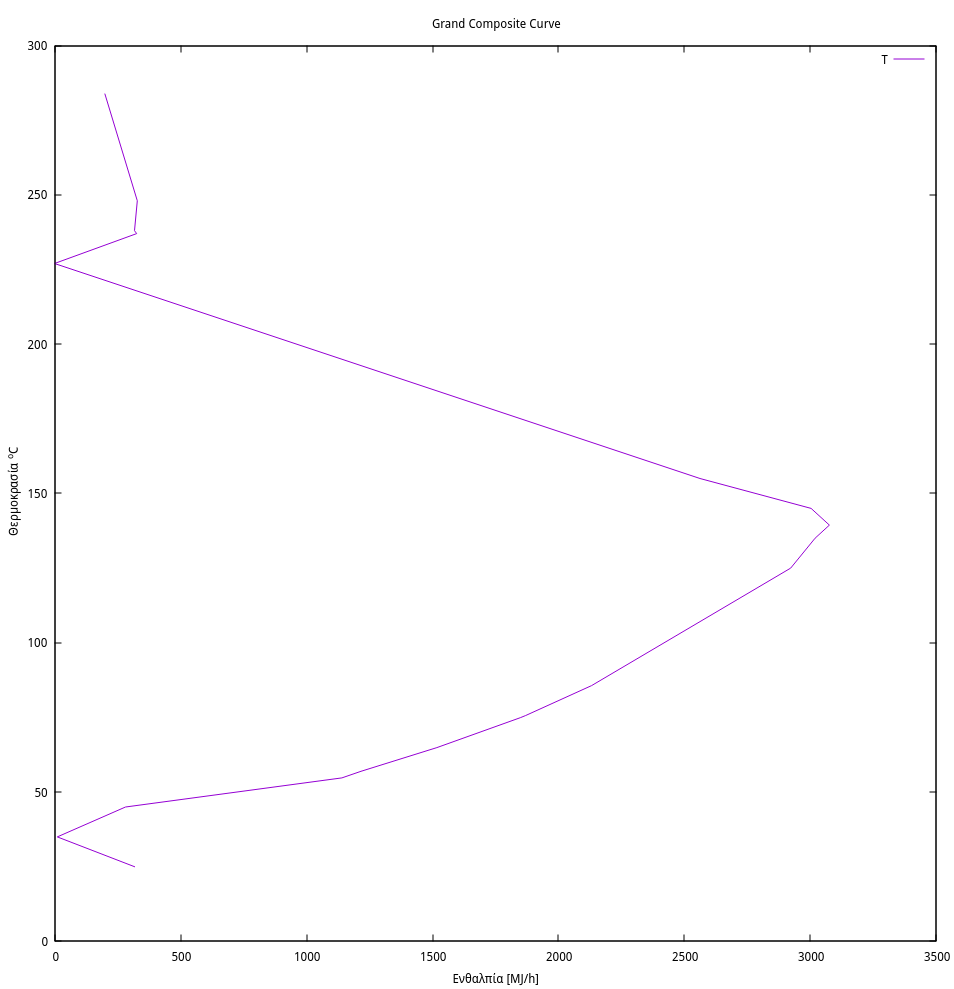
\includegraphics[width=.9\linewidth]{Diagrams/grand_composite_curve_4.png}
\caption{Μεγάλο Σύνθετο Γράφημα μετά την ολοκλήρωση 2 διεργασιών}
\end{figure}

Έχοντας το ΜΣΓ αυτό, μπορούμε να προχωρήσουμε στο σχεδιασμό του κατάλληλου δικτύου εναλλαγής θερμότητας το οποίο θα έχει η διεργασία. Αυτό όμως θα γίνει σε επόμενο στάδιο.

\pagebreak

\subsubsection{Απαίτηση σε θερμές παροχές}
\label{sec:org4fd5781}
Ιδιαίτερο ενδιαφέρον έχει να δούμε πόση ποσότητα ατμού χρειάζεται και σε τι επίπεδα χρειάζεται αυτή. Αυτό είναι ενδιαφέρον επειδή ο ατμός παράγεται από ενσωματωμένο κύκλο Rankine της διεργασίας, άρα μπορούν να επιλεχθούν τα επίπεδα κατάλληλα ανάλογα με τις απαιτήσεις. Η υψηλότερη στάθμη του ατμού είναι αρκετά υψηλή, άρα σίγουρα μπορούν να καλυφθούν όλες οι ανάγκες. Επίσης, πρέπει να ληφθεί υπόψην πως λόγω του κόστους των στροβίλων, είναι σπανίως οικονομικά επιθυμητό να έχουμε πάνω από 3 στρόβιλους στο κύκλο, άρα πάνω από 4 επίπεδα ατμού.

\begin{table}[htbp]
\caption{Απαιτούμενα επίπεδα ατμού}
\centering
\begin{tabular}{lrr}
Απαίτηση & Θερμότητα (MJ/hr) & Θερμοκρασία (C)\\
\hline
ΜΣΓ & 199.82 & 250\\
Αναβραστήρας Γλυκερόλης & 1105.44 & 300\\
Αναβραστήρας Κυκλοπεντανόνης & 9543.12 & 140\\
Αντιδραστήρας Σακχαροποίησης & 393.63 & 60\\
\end{tabular}
\end{table}

Από τα 4 ρεύματα αυτά, είναι εύκολο να παρατηρηθούν τα δύο επίπεδα που χρειάζονται. Το πρώτο πρέπει να είναι στους 300 \(^oC\) τουλάχιστον με θερμική δυνατότητα περίπου 1300 MJ/hr ενώ το δεύτερο πρέπει να είναι στους 140 \(^oC\) τουλάχιστον με θερμική δυνατότητα 10000 MJ/hr περίπου. 

Το 1ο επίπεδο είναι ο ατμός υψηλής πίεσης ο οποίος παράγεται από τα καυσαέρια. Για να παράγει ικανοποιητικά ποσά ενέργειας το κύκλο, πρέπει να είναι τουλάχιστον στα 100 bar, ώστε η εκτόνωση του να δώσει πολύ έργο. Ο ατμός που χρησιμοποιείται είναι στα 150 bar και 700 \(^oC\). Η πρώτη βαθμίδα εκτόνωσης τοποθετείται στα 30 bar όπου ο ατμός έχει θερμοκρασία 443 \(^oC\) και η θερμοκρασία του μειώνεται στους 364 \(^oC\). Η θερμοκρασία είναι πολύ υψηλή διότι ξεκινάμε από ατμό πολύ μεγάλης θερμοκρασίας και πίεσης και η εκτόνωση αυτή οδηγεί σε αυτήν την θερμοκρασία. Όμως, αυτό είναι καλό επειδή σημαίνει ότι και μετά την θέρμανση που πρέπει να κάνει, είναι ακόμη υπέρθερμος με σχετικά μεγάλο βαθμό υπερθέρμανσης άρα μπορεί να τοποθετηθεί ασφαλώς σε δεύτερο στρόβιλο όπου θα εκτονωθεί μέχρι τα 4 bar και θερμοκρασία 151 \(^oC\) ώστε να καλύψει τις ανάγκες που χρειάζονται σε χαμηλή θερμοκρασία. Η ποσότητα που χρησιμοποιήθηκε επαρκεί ώστε ο ατμός να φτάσει σε μίγμα με την υγρή φάση ποιότητας 0.5 περίπου. Θα μπορούσαμε να τραβήξουμε μικρότερη ποσότητα εξαρχής, αλλά κινδυνεύουμε να δημιουργηθεί υγρή φάση μέσα στον στρόβιλο (καθώς το νερό είναι κοντά στον κορεσμό του ως έχει) και επίσης, δυσχεραίνουμε την αναθέρμανση η οποία γίνεται με τον υπόλοιπο ατμό στα 30 bar. Η τέταρτη βαθμίδα είναι το νερό χαμηλής πίεσης που τροφοδοτούμε, το οποίο έχει πίεση 0.1 bar.

\section{Κοστολόγηση}
\label{sec:org161218a}
Πραγματοποιήθηκε οικονομική ανάλυση για τα 7 blocks της διεργασίας. Τα
αποτελέσματα αυτής συνοψίζονται στον παρακάτω πίνακα (σε χιλίαδες ευρώ). Ο πίνακας δείχνει το συνολικό κόστος κεφαλαίου, το συνολικό
κόστος λειτουργίας ανά έτος, το συνολικό κόστος πρώτων υλών ανά έτος,
τις συνολικές πωλήσεις προϊόντων ανά έτος, το συνολικό κόστος παροχών
ανά έτος, το κόστος εξοπλισμού, και το συνολικό κόστος εγκατάστασης για
κάθε διεργασία.

\begin{longtable}{rrrrr}
\caption{Συνολική Οικονομική Ανάλυση Εγκατάστασης}
\\
\hline
Blocks & Capital Cost & Operating Cost & Raw Materials Cost & Product Sales\\
100-200 & 4.281 & 8.449 & 6.645 & 0\\
300 & 3.233 & 2.277 & 0 & 0\\
400-500 & 4.061 & 2.667 & 0 & 8.857\\
600-700 & 4.287 & 4.167 & 2.573 & 83.382\\
Total & 15.862 & 17.561 & 9.218 & 92.238\\
 &  &  &  & \\
 & Ετήσιο Κέρδος & 55.992 &  & \\
\hline
\endfirsthead
\multicolumn{5}{l}{Continued from previous page} \\

 & Ετήσιο Κέρδος & 55.992 &  &  \\

\hline
\endhead
\hline\multicolumn{5}{r}{Continued on next page} \\
\endfoot
\endlastfoot
\hline
Blocks & Utilities Cost & Equipment Cost & Total Installed Cost & \\
100-200 & 78 & 488 & 1.581 & \\
300 & 1.301 & 629 & 1.101 & \\
400-500 & 1.373 & 393 & 1.349 & \\
600-700 & 71 & 890 & 1.709 & \\
Total & 2.823 & 2.399 & 5.739 & \\
 &  &  &  & \\
 & Kόστος εγκατάστασης & 8.138 &  & \\
\hline
\end{longtable}

Το συνολικό κόστος εγκατάστασης του εξοπλισμού ανέρχεται στα 8
εκατομμύρια ευρώ και το ετήσιο κέρδος είναι 56 εκατομμύρια €. Με βάση
αυτά τα αποτελέσματα, φαίνεται ότι η διεργασία αποφέρει σημαντικά έσοδα,
γεγονός που αποτελεί θετικό παράγοντα για την οικονομική βιωσιμότητα του
έργου. Το σχετικά χαμηλό κόστος των βοηθητικών παροχών, λόγω της
δυνατότητας παραγωγής τους μέσα από την διεργασία, είναι επίσης ένας θετικός
παράγοντας. Ωστόσο, το κόστος των πρώτων υλών παραμένει υψηλό οπότε θα
μπορούσε να γίνει περαιτέρω έρευνα για να διαπιστωθεί εάν υπάρχουν
ευκαιρίες για βελτιστοποίηση της διαδικασίας και μείωση του κόστους.

Τα αποτελέσματα αυτά, όμως, δεν είναι τελείως έγκυρα διότι υπάρχουν errors
στην κοστολόγηση του Aspen σε κάποια σημεία και αυτά θα πρέπει να διορθωθούν.

\subsection{Προεπεξεργασία (Blocks 100-200)}
\label{sec:orgcaf74f4}
Σε αυτό τα δύο blocks γίνεται η προεπεξεργασία του πυρηνόξυλου για την παραγωγή των τριών πλατφόρμων, γλυκόζη, ξυλόζη και λιγνίνη. Οι πρώτες ύλες που χρησιμοποιούνται είναι το
πυρηνόξηλο, το οποίο είναι απόβλητο και θεωρούμε πως παρέχεται δωρεάν, το νερό, με τιμή
0,0005488 \$/kg και το NaOH που κοστίζει 0,5\$/kg. Συνολικά, το κόστος των
πρώτων υλών είναι 6,6 εκατομμύρια ευρώ. Από τον προηγούμενο πίνακα φαίνεται ότι
για την εγκατάσταση του εξοπλισμού απαιτούνται 2.068.528 €. Θεωρούμε ότι
οι πωλήσεις των προϊόντων είναι 0 € διότι τα προϊόντα αποτελούν πλατφόρμες τις εγκατάστασης και όχι τελικά προιόντα.

\begin{longtable}{lr}
\caption{Κοστολόγηση εξοπλισμού για την προεπεξεργασία πυρηνόξυλου}
\\
Summary & \\
\hline
\endfirsthead
\multicolumn{2}{l}{Continued from previous page} \\
\hline

Summary &  \\

\hline
\endhead
\hline\multicolumn{2}{r}{Continued on next page} \\
\endfoot
\endlastfoot
\hline
Total Capital Cost [Euro] & 4.280.843\\
Total Operating Cost [Euro/Year] & 8.449.050\\
Total Raw Materials Cost [Euro/Year] & 6.644.948\\
Total Product Sales [Euro/Year] & 0\\
Total Utilities Cost [Euro/Year] & 78.161\\
Desired Rate of Return [Percent/'Year] & 18\\
P.O. Period [Year] & 0\\
Equipment Cost [Euro] & 487.876\\
Total Installed Cost [Euro] & 1.580.652\\
\end{longtable}

Στη συνέχεια παρουσιάζονται πίνακες με την κοστολόγηση κάθε εξοπλισμού
της διεργασίας, το κόστος των βοηθητικών παροχών και τα σχεδιαστικά
χαρακτηριστικά του εξοπλισμού.

\begin{longtable}{lrrl}
\caption{Κοστολόγηση εξοπλισμού}
\\
Equipment &  &  & \\
\hline
\endfirsthead
\multicolumn{4}{l}{Continued from previous page} \\
\hline

Equipment &  &  &  \\

\hline
\endhead
\hline\multicolumn{4}{r}{Continued on next page} \\
\endfoot
\endlastfoot
\hline
Name & Equipment Cost [Euro] & Installed Cost [Euro] & Equipment Weight [Kg]\\
H-101 & 104604 & 386492 & 13698,4784\\
H-103 & 8648 & 65044 & 254,01152\\
O-103 & 15548 & 114540 & 1179,3392\\
O-102 & 0 & 0 & 0\\
B1 & 0 & 0 & 0\\
O-104 & 0 & 0 & 0\\
M-201 & 0 & 0 & 0\\
C-201 & 128984 & 171948 & 2131,8824\\
H-201 & 8648 & 65044 & 254,01152\\
O-101 & 52900 & 194120 & 1950,4456\\
M-101 & 0 & 0 & 0\\
H-202 & 15548 & 87860 & 1406,1352\\
H-102 & 11040 & 84640 & 635,0288\\
P-101 & 44712 & 74244 & 1043,2616\\
R-201 & 81696 & 222180 & 3946,2504\\
E-101 & 15548 & 114540 & 1179,3392\\
\hline
Name & Installed Weight [Kg] &  & \\
H-101 & 31956,46358 &  & \\
H-103 & 3689,517328 &  & \\
O-103 & 6364,802944 &  & \\
O-102 & 0 &  & \\
B1 & 0 &  & \\
O-104 & 0 &  & \\
M-201 & 0 &  & \\
C-201 & 4186,65416 &  & \\
H-201 & 3689,517328 &  & \\
O-101 & 9547,658008 &  & \\
M-101 & 0 &  & \\
H-202 & 6857,857448 &  & \\
H-102 & 7114,59052 &  & \\
P-101 & 2193,11732 &  & \\
R-201 & 11241,37054 &  & \\
E-101 & 6364,802944 &  & \\
\end{longtable}

\begin{longtable}{llllll}
\caption{Κόστος βοηθητικών παροχών}
\\
Utilities &  &  &  &  & \\
\hline
\endfirsthead
\multicolumn{6}{l}{Continued from previous page} \\
\hline

Utilities &  &  &  &  &  \\

\hline
\endhead
\hline\multicolumn{6}{r}{Continued on next page} \\
\endfoot
\endlastfoot
\hline
Name & Fluid & Rate & Rate Units & Cost per Hour & Cost Units\\
Electricity &  & 125,055 & KW & 9,691763 & USD/H\\
\end{longtable}

\begin{longtable}{llllll}
\caption{Eναλλάκτες θερμότητας}
\\
TEMA HEX &  &  &  &  & \\
\hline
\endfirsthead
\multicolumn{6}{l}{Continued from previous page} \\
\hline

TEMA HEX &  &  &  &  &  \\

\hline
\endhead
\hline\multicolumn{6}{r}{Continued on next page} \\
\endfoot
\endlastfoot
\hline
\textbf{User tag number} & \textbf{H-101} & \textbf{H-103} & \textbf{H-201} & \textbf{H-202} & \textbf{H-102}\\
Number of identical items & 1 & 1 & 1 & 1 & 1\\
Heat transfer area [sqm] & 340,976 & 2,979083 & 2,979083 & 48,90696 & 14,46969\\
Front end TEMA symbol & B & B & B & B & B\\
Shell TEMA symbol & E & E & E & E & E\\
Rear end TEMA symbol & M & M & M & M & M\\
Tube design gauge pressure [barg] & 28,43421 & 18,61838 & 18,61838 & 0,020961 & 18,61838\\
Tube design temperature [C] & 392,5778 & 259,7778 & 256,8764 & 121,1111 & 259,7778\\
Tube operating temperature [C] & 232 & 45 & 48 & 44,93438 & 170,4094\\
Tube outside diameter [meter] & 0,0254 & 0,0254 & 0,0254 & 0,0254 & 0,0254\\
Shell design gauge pressure [barg] & 42,43421 & 28,43421 & 28,43421 & 0,020961 & 28,43421\\
Shell design temperature [C] & 392,5778 & 259,7778 & 256,8764 & 121,1111 & 259,7778\\
Shell operating temperature [C] & 364,8 & 232 & 229,0986 & 50 & 232\\
Tube length extended [meter] & 6,096 & 6,096 & 6,096 & 6,096 & 6,096\\
Tube pitch [meter] & 0,03175 & 0,03175 & 0,03175 & 0,03175 & 0,03175\\
Number of tube passes & 1 & 1 & 1 & 1 & 1\\
Number of shell passes & 1 & 1 & 1 & 1 & 1\\
\end{longtable}

\begin{longtable}{lll}
\caption{Δοχεία διαχωρισμού}
\\
Vertical vessel &  & \\
\hline
\endfirsthead
\multicolumn{3}{l}{Continued from previous page} \\
\hline

Vertical vessel &  &  \\

\hline
\endhead
\hline\multicolumn{3}{r}{Continued on next page} \\
\endfoot
\endlastfoot
\hline
\textbf{User tag number} & \textbf{O-103} & \textbf{E-101}\\
Liquid volume [l] & 2401,933 & 2401,933\\
Vessel diameter [meter] & 0,9144 & 0,9144\\
Vessel tangent to tangent height [meter] & 3,6576 & 3,6576\\
Design gauge pressure [barg] & 1,03425 & 1,03425\\
Vacuum design gauge pressure [barg] & -1,00667 & -1,00667\\
Design temperature [C] & 121,1111 & 121,1111\\
Operating temperature [C] & 69,90314 & 80,64995\\
\end{longtable}

\begin{longtable}{lll}
\caption{Διηθήσεις}
\\
Tubular filter &  & \\
\hline
\endfirsthead
\multicolumn{3}{l}{Continued from previous page} \\
\hline

Tubular filter &  &  \\

\hline
\endhead
\hline\multicolumn{3}{r}{Continued on next page} \\
\endfoot
\endlastfoot
\hline
\textbf{User tag number} & \textbf{O-102} & \textbf{O-104}\\
Liquid flow rate [l/min] & 26,52002 & 17,94001\\
\end{longtable}

\begin{longtable}{lrrr}
\caption{Αναμιχτήρες}
\\
Quoted equipment &  &  & \\
\hline
\endfirsthead
\multicolumn{4}{l}{Continued from previous page} \\
\hline

Quoted equipment &  &  &  \\

\hline
\endhead
\hline\multicolumn{4}{r}{Continued on next page} \\
\endfoot
\endlastfoot
\hline
\textbf{User tag number} & \textbf{B1} & \textbf{M-201} & \textbf{M-101}\\
Code of account & 100 & 100 & 100\\
Material cost per unit & 0 & 0 & 0\\
\end{longtable}

\begin{longtable}{lll}
\caption{Αντιδραστήρες}
\\
Agitated reactor &  & \\
\hline
\endfirsthead
\multicolumn{3}{l}{Continued from previous page} \\
\hline

Agitated reactor &  &  \\

\hline
\endhead
\hline\multicolumn{3}{r}{Continued on next page} \\
\endfoot
\endlastfoot
\hline
\textbf{User tag number} & \textbf{O-101} & \textbf{R-201}\\
Liquid volume [l] & 450,3624 & 2502,013\\
Vessel diameter [meter] & 0,4572 & 0,9144\\
Vessel tangent to tangent height [meter] & 2,7432 & 3,81\\
Design gauge pressure [barg] & 28,43421 & 1,03425\\
Vacuum design gauge pressure [barg] &  & -1,00667\\
Design temperature [C] & 259,7778 & 121,1111\\
\end{longtable}

\begin{longtable}{ll}
\caption{Αντλία}
\\
Centrif pump & \\
\hline
\endfirsthead
\multicolumn{2}{l}{Continued from previous page} \\
\hline

Centrif pump &  \\

\hline
\endhead
\hline\multicolumn{2}{r}{Continued on next page} \\
\endfoot
\endlastfoot
\hline
\textbf{User tag number} & \textbf{P-101}\\
Liquid flow rate [l/min] & 216,678\\
Fluid head [meter] & 264,5286\\
Fluid specific gravity & 0,965073\\
Design gauge pressure [barg] & 28,43421\\
Design temperature [C] & 21,11111\\
Fluid viscosity [cP] & 0,5\\
Pump efficiency [fraction] & 0,445604\\
\end{longtable}

\subsection{Κύκλο Rankine (Block 300)}
\label{sec:orgb6a36fd}
Κατά την κοστολόγηση της μονάδας αυτής προέκυψαν αρκετά errors για αυτό η πρώτη εικόνα της κοστολόγησης που αναφέρεται στο αρχείο αυτό δεν τα συμπεριλαμβάνει. Άρα το κέρδος θα είναι χαμηλότερο λόγω του ακριβού εξοπλισμού της (κυρίως τους 3 στρόβιλους), όμως επειδή παράγει όλες τις απαιτούμενες θερμές παροχές της διεργασίας και μία πολύ μεγαλύτερη από την απαιτούμενη ποσότητα ηλεκτρισμού (ο οποίος μπορεί να μεταπωληθεί) θεωρείται πως θα έχει θετικό ισοζύγιο.

\subsection{Παραγωγή και Καθαρισμός Γλυκερόλης (Blocks 400-500)}
\label{sec:org52ee46b}
Έγινε οικονομική αξιολόγηση των blocks 400-500, με τελικό προιόν την
γλυκερόλη με καθαρότητα 99,96\% σε ποσότητα 12845 tn/year. Βρέθηκε
πως η τιμή αγοράς γλυκερόλης σε υψηλή καθαρότητα μπορεί να πουληθεί
για 0,34 \$/lb ή 0,732 euro/kg.

Επίσης έγινε και διαστασιολόγηση του εξοπλισμού και οικονομική ανάλυση
των παροχών που απαιτούνται. Μια σύντομη περιγραφή των αποτελεσμάτων
παρουσιάζονται στον παρακάτω πίνακα. Η παρούσα οικονομική ανάλυση
ασχολείται με τις διεργασίες που χρησιμοποιούνται από την έξοδο του
βιοαντιδραστήρα και μετά, συνεπώς δεν αγοράζεται κάποια πρώτη ύλη.

\begin{longtable}{lr}
\caption{Συνολικό κόστος διεργασίας}
\\
Summary & \\
\hline
\endfirsthead
\multicolumn{2}{l}{Continued from previous page} \\
\hline

Summary &  \\

\hline
\endhead
\hline\multicolumn{2}{r}{Continued on next page} \\
\endfoot
\endlastfoot
\hline
Total Capital Cost [kEuro] & 4061\\
Total Operating Cost [kEuro/Year] & 2667\\
Total Product Sales [kEuro/Year] & 8856\\
Total Utilities Cost [kEuro/Year] & 1373\\
Desired Rate of Return [Percent/'Year] & 18,4\\
P.O. Period [Year] & 1,9336\\
Equipment Cost [kEuro] & 392\\
Total Installed Cost [kEuro] & 1349\\
\end{longtable}

Συνεπώς για την εγκατάσταση αυτού του εξοπλισμού απαιτούνται 1741,744
kEuro, και αφού ξεκινήσει να λειτουργεί αυτή η θα έχει συνολικό ετήσιο
κέρδος της τάξεως των 755,2372 kEuro/y, που σημαίνει ότι θα χρειαστούν
γύρω στα 2,3 χρόνια για να γίνει απόσβεση του κόστους εγκατάστασης αυτών
των διεργασιών.

Παρουσιάζεται πίνακας με την αναλυτική κοστολόγηση κάθε εξοπλισμού της
διεργασίας

\begin{longtable}{llrl}
\caption{Αναλυτική Κοστολόγηση Εξοπλισμού}
\\
\hline
Name & Equipment Cost [Euro] & Installed Cost [Euro] & Equipment Weight [Kg]\\
\hline
\endfirsthead
\multicolumn{4}{l}{Continued from previous page} \\
\hline

Name & Equipment Cost [Euro] & Installed Cost [Euro] & Equipment Weight [Kg] \\

\hline
\endhead
\hline\multicolumn{4}{r}{Continued on next page} \\
\endfoot
\endlastfoot
\hline
H-502 & 23368 & 120520 & 2540,1152\\
C-501 & 128984 & 171948 & 2131,8824\\
H-501 & 8372 & 65228 & 231,33192\\
H-503 & 25392 & 124936 & 2857,6296\\
R-401 & 81236 & 221536 & 3810,1728\\
D-501-cond & 7728 & 50508 & 117,93392\\
D-501-cond acc & 15180 & 105248 & 1224,6984\\
D-501-reb & 40388 & 118036 & 4490,5608\\
D-501-reflux pump & 4416 & 27876 & 90,7184\\
D-501-tower & 33672 & 172224 & 2313,3192\\
F-501-flash vessel & 23828 & 171120 & 2086,5232\\
\hline
Name & Installed Weight [Kg] &  & \\
\hline
H-502 & 12602,60013 &  & \\
C-501 & 4186,65416 &  & \\
H-501 & 3777,514176 &  & \\
H-503 & 13640,41862 &  & \\
R-401 & 11077,62382 &  & \\
D-501-cond & 2105,120472 &  & \\
D-501-cond acc & 5870,841256 &  & \\
D-501-reb & 9960,426728 &  & \\
D-501-reflux pump & 1126,268936 &  & \\
D-501-tower & 9538,132576 &  & \\
F-501-flash vessel & 11794,75278 &  & \\
\hline
\end{longtable}

\begin{longtable}{llllll}
\caption{Κοστολόγηση βοηθητικών παροχών}
\\
Utilities &  &  &  &  & \\
\hline
\endfirsthead
\multicolumn{6}{l}{Continued from previous page} \\
\hline

Utilities &  &  &  &  &  \\

\hline
\endhead
\hline\multicolumn{6}{r}{Continued on next page} \\
\endfoot
\endlastfoot
\hline
Name & Fluid & Rate & Rate Units & Cost per Hour & Cost Units\\
Electricity &  & 97,173 & KW & 6,92843444 & Euro/H\\
Cooling Water & Water & 0,00085 & MMGAL/H & 0,09384 & Euro/H\\
Steam @100PSI & Steam & 19,97789 & KLB/H & 149,610423 & Euro/H\\
\end{longtable}

Η οικονομική ανάλυση για τις βοηθητικές παροχές που παρουσιάζεται εδώ,
αποτελεί την περίπτωση όπου το block 300 της συνολικής διεργασίας δεν αρκεί για να τις
καλύψει, παρόλο που προσφέρει μεγάλες ποσότητες ηλεκτρικής ενέργειας
και θερμών παροχών. Συνεπώς αυτή η οικονομική ανάλυση αποτελεί ένα worst
case scenario όσον αφορά την ηλεκτρική ενέργεια και τις θερμές παροχές,
ενώ η ανάλυση για τις ψυχρές παραμένει έγκυρη.

Παρουσιάζονται πίνακες για τα σχεδιαστικά χαρακτηριστικά του εξοπλισμού
που προέκυψαν από την διαστασιολόγηση.


\begin{longtable}{lllll}
\caption{Διαστασιολόγηση Εναλλακτών Θερμότητας}
\\
\textbf{TEMA HEX} &  &  &  & \\
\hline
\endfirsthead
\multicolumn{5}{l}{Continued from previous page} \\
\hline

\textbf{TEMA HEX} &  &  &  &  \\

\hline
\endhead
\hline\multicolumn{5}{r}{Continued on next page} \\
\endfoot
\endlastfoot
\hline
\textbf{User tag number} & \textbf{H-502} & \textbf{H-501} & \textbf{H-503} & \textbf{D-501-cond}\\
Number of identical items & 1 & 1 & 1 & 1\\
Heat transfer area [sqm] & 91,5801 & 2,557231 & 110,8726 & 0,382876279\\
Front end TEMA symbol & B & B & B & B\\
Shell TEMA symbol & E & E & E & E\\
Rear end TEMA symbol & M & M & M & M\\
Tube design gauge pressure [barg] & 0,020961 & 1,285044 & 7,605461 & 4,1579608\\
Tube design temperature [C] & 167,789 & 316,71 & 192,1111 & 243,5217839\\
Tube operating temperature [C] & 95 & 44 & 164,3333 & 35\\
Tube outside diameter [meter] & 0,0254 & 0,0254 & 0,0254 & 0,0254\\
Shell design gauge pressure [barg] & 0,020961 & 2,434211 & 4,732544 & 2,4342108\\
Shell design temperature [C] & 167,789 & 316,71 & 167,7778 & 243,5217839\\
Shell operating temperature [C] & 140,0112 & 288,9322 & 140 & 215,7440061\\
Tube length extended [meter] & 6,096 & 6,096 & 6,096 & 6,096\\
Tube pitch [meter] & 0,03175 & 0,03175 & 0,03175 & 0,03175\\
Number of tube passes & 1 & 1 & 1 & 1\\
Number of shell passes & 1 & 1 & 1 & 1\\
\end{longtable}

\begin{longtable}{ll}
\caption{Διαστασιολόγηση φυγοκέντρου}
\\
\textbf{Solid bowl centrif} & \\
\hline
\endfirsthead
\multicolumn{2}{l}{Continued from previous page} \\
\hline

\textbf{Solid bowl centrif} &  \\

\hline
\endhead
\hline\multicolumn{2}{r}{Continued on next page} \\
\endfoot
\endlastfoot
\hline
\textbf{User tag number} & \textbf{C-501}\\
Remarks 1 & Equipment mapped from 'C-501'.\\
Bowl diameter [meter] & 0,4572\\
Bowl length [meter] & 1,016\\
Flow rate [kg/hr] & 1874,336\\
\end{longtable}


\begin{longtable}{ll}
\caption{Διαστασιολόγηση συμπηκνωτή αποστακτικής στήλης}
\\
\textbf{Horizontal drum} & \\
\hline
\endfirsthead
\multicolumn{2}{l}{Continued from previous page} \\
\hline

\textbf{Horizontal drum} &  \\

\hline
\endhead
\hline\multicolumn{2}{r}{Continued on next page} \\
\endfoot
\endlastfoot
\hline
\textbf{User tag number} & \textbf{D-501-cond acc}\\
Remarks 1 & Equipment mapped from 'D-501'.\\
Liquid volume [l] & 1801,449698\\
Vessel diameter [meter] & 0,9144\\
Vessel tangent to tangent length [meter] & 2,7432\\
Design gauge pressure [barg] & 1,03425\\
Vacuum design gauge pressure [barg] & -1,00667\\
Design temperature [C] & 172,1626089\\
Operating temperature [C] & 144,3848311\\
\end{longtable}


\begin{longtable}{ll}
\caption{Διαστασιολόγηση αναθερμαντή αποστακτικής στήλης}
\\
\textbf{U-tube reboiler} & \\
\hline
\endfirsthead
\multicolumn{2}{l}{Continued from previous page} \\
\hline

\textbf{U-tube reboiler} &  \\

\hline
\endhead
\hline\multicolumn{2}{r}{Continued on next page} \\
\endfoot
\endlastfoot
\hline
\textbf{User tag number} & \textbf{D-501-reb}\\
Remarks 1 & Equipment mapped from 'D-501'.\\
Number of identical items & 1\\
Heat transfer area [sqm] & 140,2956413\\
Tube design gauge pressure [barg] & 1,28504411\\
Tube design temperature [C] & 343,3333333\\
Tube operating temperature [C] & 288,9322461\\
Tube outside diameter [meter] & 0,0254\\
Shell design gauge pressure [barg] & 2,4342108\\
Shell design temperature [C] & 343,3333333\\
Shell operating temperature [C] & 315,5555556\\
Tube length extended [meter] & 6,096\\
Tube pitch [meter] & 0,03175\\
Tube pitch symbol & TRIANGULAR\\
Number of tube passes & 2\\
Duty [cal/sec] & 73342,06549\\
TEMA type & BKU\\
\end{longtable}


\begin{longtable}{ll}
\caption{Διαστασιολόγηση αντλίας αποστακτικής στήλης}
\\
\textbf{Centrif pump} & \\
\hline
\endfirsthead
\multicolumn{2}{l}{Continued from previous page} \\
\hline

\textbf{Centrif pump} &  \\

\hline
\endhead
\hline\multicolumn{2}{r}{Continued on next page} \\
\endfoot
\endlastfoot
\hline
\textbf{User tag number} & \textbf{D-501-reflux pump}\\
Remarks 1 & Equipment mapped from 'D-501'.\\
Liquid flow rate [l/min] & 1,78125534\\
Fluid specific gravity & 1,159661\\
Design gauge pressure [barg] & 1,03425\\
Design temperature [C] & 172,1626089\\
Fluid viscosity [cP] & 0,5\\
Pump efficiency [fraction] & 0,7\\
\end{longtable}


\begin{longtable}{ll}
\caption{Διαστασιολόγηση αποστακτικής στήλης}
\\
\textbf{Multi-diameter tower} & \\
\hline
\endfirsthead
\multicolumn{2}{l}{Continued from previous page} \\
\hline

\textbf{Multi-diameter tower} &  \\

\hline
\endhead
\hline\multicolumn{2}{r}{Continued on next page} \\
\endfoot
\endlastfoot
\hline
\textbf{User tag number} & \textbf{D-501-tower}\\
Remarks 1 & Equipment mapped from 'D-501'.\\
Diameter Bottom section [meter] & 0,6096\\
Bottom tangent to tangent height [meter] & 7,3152\\
Design gauge pressure Bottom [barg] & 2,4342108\\
Design temperature Bottom [C] & 316,7100239\\
Operating temperature Bottom [C] & 288,9322461\\
Number of trays Bottom section & 6\\
Bottom Tray type & SIEVE\\
Bottom Tray spacing [meter] & 0,6096\\
Molecular Wt Overhead Prod. & 92,068115\\
\end{longtable}


\begin{longtable}{ll}
\caption{Διαστασιολόγηση του Flash διαχωριστήρα}
\\
\textbf{Vertical vessel} & \\
\hline
\endfirsthead
\multicolumn{2}{l}{Continued from previous page} \\
\hline

\textbf{Vertical vessel} &  \\

\hline
\endhead
\hline\multicolumn{2}{r}{Continued on next page} \\
\endfoot
\endlastfoot
\hline
\textbf{User tag number} & \textbf{F-501-flash vessel}\\
Remarks 1 & Equipment mapped from 'F-501'.\\
Liquid volume [l] & 8073,163475\\
Vessel diameter [meter] & 1,6764\\
Vessel tangent to tangent height [meter] & 3,6576\\
Design gauge pressure [barg] & 1,03425\\
Design temperature [C] & 167,7777778\\
Operating temperature [C] & 140\\
\end{longtable}

\subsection{Παραγωγή και Καθαρισμός Κυκλοπεντανόνης (Blocks 600-700)}
\label{sec:org2a8ddd1}
Σε αυτή τη μονάδα γίνεται παραγωγή 19615 tn/yr κυκλοπεντανόνης με
καθαρότητα 98\%, η οποία μπορεί να πωληθεί στην αγορά σε τιμή 5 \$/kg. Οι
πρώτες ύλες που χρησιμοποιούνται για την παραγωγή κυκλοπεντανόνης είναι
η ξυλόζη, η οποία θεωρήθηκε δωρεάν επειδή είναι προϊόν από την
επεξεργασία της βιομάζας, το νερό για το οποίο ορίστηκε η τιμή 0,0005488
\$/kg και το υδρογόνο, το οποίο κοστίζει 2 \$/kg. Όπως φαίνεται στον παρακάτω πίνακα, η εγκατάσταση του εξοπλισμού θα κοστίσει 2.599.092 € και
μόλις τεθεί σε λειτουργία, αναμένεται να αποφέρει ετήσιο κέρδος
74.856.185 €.

\begin{longtable}{lr}
\caption{Σύνοψη Κοστολόγησης}
\\
Summary & \\
\hline
\endfirsthead
\multicolumn{2}{l}{Continued from previous page} \\
\hline

Summary &  \\

\hline
\endhead
\hline\multicolumn{2}{r}{Continued on next page} \\
\endfoot
\endlastfoot
\hline
Total Capital Cost [Euro] & 4.287.090\\
Total Operating Cost [Euro/Year] & 4.167.140\\
Total Raw Materials Cost [Euro/Year] & 2.572.826\\
Total Product Sales [Euro/Year] & 83.381.808\\
Total Utilities Cost [Euro/Year] & 71.393\\
Desired Rate of Return [Percent/'Year] & 18\\
P.O. Period [Year] & 0\\
Equipment Cost [Euro] & 890.376\\
Total Installed Cost [Euro] & 1.708.716\\
\end{longtable}

Ακολουθούν πίνακες με την κοστολόγηση του εξοπλισμού και των βοηθητικών
παροχών, και τα σχεδιαστικά χαρακτηριστικά του εξοπλισμού.

\begin{longtable}{lrrr}
\caption{Κοστολόγηση Εξοπλισμού για την παραγωγή Κυκλοπεντανόνης}
\\
Equipment &  &  & \\
\hline
\endfirsthead
\multicolumn{4}{l}{Continued from previous page} \\
\hline

Equipment &  &  &  \\

\hline
\endhead
\hline\multicolumn{4}{r}{Continued on next page} \\
\endfoot
\endlastfoot
\hline
Name & Equipment Cost [Euro] & Installed Cost [Euro] & Equipment Weight [Kg]\\
H2 & 8.556 & 65.504 & 245\\
REMOVAL & 24.748 & 105.064 & 3.447\\
R-CYCL & 206.448 & 370.116 & 18.461\\
R-FURF & 44.988 & 177.468 & 1.542\\
COL1 & 592.480 & 885.316 & 130.861\\
FEEDTURB & 4.600 & 33.856 & 132\\
H1 & 8.556 & 71.392 & 245\\
\hline
Name & Installed Weight [Kg] &  & \\
H2 & 3.817 &  & \\
REMOVAL & 8.433 &  & \\
R-CYCL & 28.585 &  & \\
R-FURF & 8.214 &  & \\
COL1 & 151.142 &  & \\
FEEDTURB & 1.775 &  & \\
H1 & 5.047 &  & \\
\end{longtable}

\begin{longtable}{llllll}
\caption{Κόστη βοηθητικών παροχών}
\\
Utilities &  &  &  &  & \\
\hline
\endfirsthead
\multicolumn{6}{l}{Continued from previous page} \\
\hline

Utilities &  &  &  &  &  \\

\hline
\endhead
\hline\multicolumn{6}{r}{Continued on next page} \\
\endfoot
\endlastfoot
\hline
Name & Fluid & Rate & Rate Units & Cost per Hour & Cost Units\\
Electricity &  & 104,54 & KW & 8,10185 & USD/H\\
Cooling Water & Water & 0,006256 & MMGAL/H & 0,75072 & USD/H\\
\end{longtable}

\begin{longtable}{lll}
\caption{Εναλλάκτες Θερμότητας}
\\
\textbf{TEMA HEX} &  & \\
\hline
\endfirsthead
\multicolumn{3}{l}{Continued from previous page} \\
\hline

\textbf{TEMA HEX} &  &  \\

\hline
\endhead
\hline\multicolumn{3}{r}{Continued on next page} \\
\endfoot
\endlastfoot
\hline
\textbf{User tag number} & \textbf{H2} & \textbf{H1}\\
Number of identical items & 1 & 1\\
Heat transfer area [sqm] & 2,759166 & 1,845522\\
Front end TEMA symbol & B & B\\
Shell TEMA symbol & E & E\\
Rear end TEMA symbol & M & M\\
Tube design gauge pressure [barg] & 10,67368 & 28,43421\\
Tube design temperature [C] & 269,7778 & 343,3333\\
Tube operating temperature [C] & 35 & 243\\
Tube outside diameter [meter] & 0,0254 & 0,0254\\
Shell design gauge pressure [barg] & 16,51716 & 18,61838\\
Shell design temperature [C] & 269,7778 & 343,3333\\
Shell operating temperature [C] & 242 & 315,5556\\
Tube length extended [meter] & 6,096 & 6,096\\
Tube pitch [meter] & 0,03175 & 0,03175\\
Number of tube passes & 1 & 1\\
Number of shell passes & 1 & 1\\
\end{longtable}

\begin{longtable}{ll}
\caption{Flash}
\\
Vertical vessel & \\
\hline
\endfirsthead
\multicolumn{2}{l}{Continued from previous page} \\
\hline

Vertical vessel &  \\

\hline
\endhead
\hline\multicolumn{2}{r}{Continued on next page} \\
\endfoot
\endlastfoot
\hline
\textbf{User tag number} & \textbf{REMOVAL}\\
Liquid volume [l] & 3269,297609\\
Vessel diameter [meter] & 1,0668\\
Vessel tangent to tangent height [meter] & 3,6576\\
Design gauge pressure [barg] & 42,43421077\\
Vacuum design gauge pressure [barg] & \\
Design temperature [C] & 187,7777778\\
Operating temperature [C] & 160\\
\end{longtable}

\begin{longtable}{lll}
\caption{Αντιδραστήρας}
\\
Agitated reactor &  & \\
\hline
\endfirsthead
\multicolumn{3}{l}{Continued from previous page} \\
\hline

Agitated reactor &  &  \\

\hline
\endhead
\hline\multicolumn{3}{r}{Continued on next page} \\
\endfoot
\endlastfoot
\hline
\textbf{User tag number} & \textbf{R-CYCL} & \textbf{R-FURF}\\
Liquid volume [l] & 13455,27248 & 375,3020224\\
Vessel diameter [meter] & 1,6764 & 0,4572\\
Vessel tangent to tangent height [meter] & 6,096 & 2,286\\
Design gauge pressure [barg] & 42,43421077 & 16,5171608\\
Vacuum design gauge pressure [barg] &  & \\
Design temperature [C] & 187,7777778 & 270,8939528\\
\end{longtable}

\begin{longtable}{ll}
\caption{Αποστακτική Στήλη}
\\
Multi-diameter tower & \\
\hline
\endfirsthead
\multicolumn{2}{l}{Continued from previous page} \\
\hline

Multi-diameter tower &  \\

\hline
\endhead
\hline\multicolumn{2}{r}{Continued on next page} \\
\endfoot
\endlastfoot
\hline
\textbf{User tag number} & \textbf{COL1}\\
Diameter Bottom section [meter] & 0,91\\
Bottom tangent to tangent height [meter] & 49,99\\
Design gauge pressure Bottom [barg] & 42,43\\
Design temperature Bottom [C] & 295,62\\
Operating temperature Bottom [C] & 267,84\\
Number of trays Bottom section & 76,00\\
Bottom Tray type & SIEVE\\
Bottom Tray spacing [meter] & 0,61\\
Molecular Wt Overhead Prod. & 19,17\\
\end{longtable}

\begin{longtable}{ll}
\caption{Στρόβιλος}
\\
Centrif pump & \\
\hline
\endfirsthead
\multicolumn{2}{l}{Continued from previous page} \\
\hline

Centrif pump &  \\

\hline
\endhead
\hline\multicolumn{2}{r}{Continued on next page} \\
\endfoot
\endlastfoot
\hline
\textbf{User tag number} & \textbf{FEEDTURB}\\
Liquid flow rate [l/min] & 73,06199902\\
Fluid specific gravity & 0,993669\\
Design gauge pressure [barg] & 16,31046077\\
Design temperature [C] & 270,8939528\\
Fluid viscosity [cP] & 0,5\\
Pump efficiency [fraction] & 0,295658\\
\end{longtable}
\end{document}